\documentclass[a4paper,12pt]{article}

%\usepackage{times}
%\usepackage[T3,T1]{fontenc}
%\usepackage[utf8x]{inputenc}
% \usepackage[T1]{fontenc}
% \usepackage{mathptmx}  

\usepackage{fontspec} %,xunicode} % xltxtra
    \defaultfontfeatures{Ligatures=TeX}
    \setmainfont{Brill}[
    Extension=.ttf,
    UprightFont=*-Roman,
    BoldFont=*-Bold,
    ItalicFont=*-Italic,
    BoldItalicFont=*-Bold-Italic,
    Renderer=ICU]
% 	\usefonttheme{serif}
%	\setmainfont[Renderer=ICU]{Charis SIL}
% 	\setmainfont[Renderer=ICU]{Brill}

%% Trigger answers and notes. Package by Byron Ahn with edits by Craig Sailor
\usepackage[solution,spaces]{myProbSol} %   Optional arguments:
%                                               'solution': reveals solutions
%                                               'spaces': leaves whitespace corresponding to the size of the solutions (has no effect if you also pass 'solution')

\usepackage{amsmath,amssymb} % for $\text{}$
\usepackage{url,natbib} 
\usepackage[dvipsnames]{xcolor} %,bm}
\usepackage{geometry,vmargin,setspace}
\usepackage{multirow}
\setmarginsrb{1in}{1in}{1in}{1in}{13.6pt}{0.1in}{0.1in}{0.2in}
% pdflscape} %rotating
    \setlength{\parindent}{0pt}

\usepackage{stmaryrd}
\usepackage{wasysym} %checkbox
\usepackage[normalem]{ulem} % for \sout{}
% \usepackage{mdwlist} % for \begin{itemize*} - but prefer \tightlist
\providecommand{\tightlist}{%
	\setlength{\itemsep}{0pt}\setlength{\parskip}{0pt}}

\usepackage{natbib}
	\bibpunct[:]{(}{)}{;}{a}{}{,}
	\setlength{\bibsep}{0pt plus 0.3ex}

\usepackage{longtable}
\usepackage[linkcolor=purple,citecolor=ForestGreen,colorlinks=true,urlcolor=gray,pagebackref=true]{hyperref}
\usepackage{multicol}
\usepackage{dashrule} %\hdashrule
\usepackage{array} % >{\...} in tabulars
\usepackage{arydshln}

\usepackage[framemethod=tikz,footnoteinside=false]{mdframed} 

\usepackage{expex} %Linguistics examples
\lingset{aboveexskip=0ex,belowexskip=0.5ex,aboveglftskip=-0.3em,interpartskip=0ex,labelwidth=!6pt,belowpreambleskip=0.1ex} %, *=*?}
%	\lingset{aboveexskip=0.5ex,belowexskip=0.5ex,*=??}

\usepackage[nocenter]{qtree} % trees
\usepackage{tikz}
    \tikzstyle{every picture}+=[remember picture]

\usepackage{tipa} % convenient for \textsubarch etc.

\newcommand\trace{\rule[-0.5ex]{0.5cm}{.4pt}}
\bibpunct[:]{(}{)}{;}{a}{}{,}
	\setlength{\bibsep}{0pt plus 0.3ex}

\usepackage{pifont}
\newcommand{\cmark}{\ding{51}}% 52
\newcommand{\xmark}{\ding{55}}%
 \newcommand{\hand}{\ding{43}}

\newcommand\zero{\O{}}
\newcommand\itp[1]{\textit{\textipa{#1}}}
\newcommand\gsc[1]{\textsc{\lowercase{#1}}} %for glossing in small caps - comment out to return to caps
\renewcommand\root[1]{$\sqrt{\text{#1}}$}

\newcommand\blue[1]{\textcolor{blue}{#1}}
\newcommand\red[1]{\textcolor{red}{#1}}
\newcommand\green[1]{\textcolor{ForestGreen}{#1}}
\newcommand\gray[1]{\textcolor{gray}{#1}}
\newcommand\denote[1]{$\llbracket$#1$\rrbracket$}
\newcommand\lra{$\leftrightarrow$}

\newcommand\vz{\text{Voice$_{\text{\{--D\}}}$}}
\newcommand\vd{\text{Voice$_{\text{\{+D\}}}$}}
\newcommand\pz{\text{$p_{\text{\zero}}$}}
\newcommand\va{\root{\gsc{ACTION}}}
\newcommand{\tkal}{\emph{XaYaZ}}
\newcommand{\tpie}{\emph{XiY̯eZ}}
\newcommand{\tpua}{\emph{XuY̯aZ}}
\newcommand{\thif}{\emph{heXYiZ}}
\newcommand{\thuf}{\emph{huXYaZ}}
\newcommand{\thit}{\emph{hitXaY̯eZ}}
\newcommand{\tnif}{\emph{niXYaZ}}
\newcommand\dgs[1]{\textsubarch{#1}}
\newcommand\del[1]{\sout{#1}}

\makeatletter %Allow superscript ^ and subscript _
\catcode`_=\active%
\gdef_#1{\ensuremath{{}\sb{#1}}}%
\catcode`^=\active%
\gdef^#1{\ensuremath{{}\sp{#1}}}%
\makeatother

\begin{document}
% \pagenumbering{gobble}
% \singlespacing


\hfill \emph{Morphology 2023-24, Edinburgh}

\section{Introduction}

    \subsection{What is morphology?}
When we study morphology, the structure of words, there is a range of things that might interest us. Some things we mentioned are:
\begin{enumerate} \tightlist
    \item Morphology's relationship to syntax (morphosyntax, and specifically syntactic features and argument structure)
    \item Morphology's relationship to phonology (morphophonology, and specifically allomorphy)
    \item Morphology's relationship to semantics (morphosemantics, and specifically lexical semantics)
    \item Lexical processing (psycholinguistics)
    \item Lexical acquisition (L1/L2)
    \item Computational modeling
    \item Lexical change (historical linguistics)
    \item Lexical variation (variationist sociolinguistics)
\end{enumerate}

How do we accurately describe how language works? We need a theory, which predicts both what does happen and what cannot ever happen. Once we have a theory in place, we can form hypotheses and test them. So for example, suppose we find that L2 learners of English learners learn the plural suffix -\emph{s} in \emph{dogs} before the agentive suffix -\emph{er} of \emph{worker}. Is this because:
\begin{itemize} \tightlist
    \item The former is more frequent in terms of total number of words (tokens)?
    \item The former is more frequent in terms of the number of distinct words it can attach to (types)?
    \item The former is conceptually easier to learn?
    \item The former is more regular in its meaning (compare \emph{worker} with \emph{computer} or \emph{ruler})?
    \item The former is inflection and the latter derivation?
    \item All/some/none of the above?
\end{itemize}

Once we have a hypothesis in place about how morphology works, we can make predictions about learning.

The questions we ask lead us to develop a variant of the framework called Distributed Morphology, or simply DM for short \citep{dm}. The core idea of DM is that morphology (words) have complex internal hierarchical structure just like syntax (sentences) does. DM actually assumes that morphology and syntax are one and the same structure. But we build up to this idea, seeing what it predicts and what we can learn along the way.

\paragraph{General readings on DM}
The course does not follow a specific textbook; there is, in fact, no current textbook which motivates the architectural assumptions of DM in the way we try to do (although the upcoming \citealt{punske23} looks promising). Here are some suggestions for general references on the framework.

\begin{itemize} \tightlist
    \item For the bare-bones version of ``what you need to know'', have a look at the introductory chapter to a recent book on morphology using DM. For example, \cite{wood15springer} and \cite{myler17oup} both have good overviews. Chapter 1.3 of \cite{kastner20ogs} has an extremely \sout{short} economical overview.
    \item For a single-article overview, I like \cite{mcginnis16cup}. \cite{harley13handbook} is particularly useful in that it does not assume that its audience knows what we're talking about. \cite{embicknoyer07} and \cite{bobaljik17oup} are both good as well, and fairly comprehensive for single-chapter overviews (especially when it comes to morphophonological details).
    \item There are one published textbook and two unpublished textbook drafts which together cover a lot of ground. The published one is \cite{embick15}. The unpublished ones are \cite{nevins16ms}, which you can find on the online repository \href{https://ling.auf.net/lingbuzz/}{LingBuzz}, and \cite{bobaljikbaker02}, which does not have one official ``home'', as far as I can tell, but which is hosted as separate PDFs on a number of sites.
    \item I would \emph{not} recommend starting with \cite{dm}, which is both very technical and slightly outdated, although it is a good read.
    \item For general textbooks on morphology, check out \cite{harley06}, which focuses on English, and \cite{fabregasscalise12}, which tries to survey different theories.
    \item There is no need to read any of these works to understand or follow what we're doing in class: we'll develop the theory together!
\end{itemize}

    \subsection{What's a word?}
We started by seeing whether we can come up with a definition of ``word'' that's consistent across all its uses. Does a ``word'' in one domain also identify a unit in another domain?

And some related questions: What elements can combine and how? What elements can stand on their own, and when? At what points in a ``word'' can we interrupt it, or interrupt the language user? What is a word? What kinds of words are there?

\begin{enumerate} \tightlist
    \item Orthographic word
        \begin{itemize} \tightlist
        \item A written element separated by spaces
        \item Nice and clear definition, useful if you don't know where to start
        \item Not all languages use spaces to separate ``words'' (Thai, Chinese)
        \item A ``word'' in one language might be different than the same ``word'' in another language
        \item Not all languages have writing systems: ancient languages, dialects and other varieties, sign languages
        \item Language existed a long time before writing was invented (and early writing systems tend not to have spaces; see also scriptio continua)
        \item In English, we have things that seem word-like but that are divided by spaces, like compounds or phrasal verbs. Sometimes we get arbitrary minimal pairs: \emph{do not} $\sim$ \emph{cannot}
        \end{itemize}
    \item Lexicographic word
        \begin{itemize} \tightlist
            \item Dictionary entry
            \item Who decides what goes in the dictionary?
            \item There's too much information: lots of words we don't know, so that's knowledge the language user doesn't necessarily have synchronically
            \item There's too little information: doesn't contain everything you could say about the entry, and is usually not up to date
            \item Tricky to decide how to organise the information: what to do with inflection (\emph{run, ran, running}) and derivation (\emph{run, runner})? Separate entries?
            \item Different dictionaries for different languages are organised differently (e.g. by roots)
        \end{itemize}
    \item Semantic word
        \begin{itemize} \tightlist
            \item Is a \emph{dog} really one thing?
            \item What about function words like \emph{the}? Function morphemes like [\textsc{plural}] or [\textsc{past}]?
            \item The meaning of deictic elements like \emph{that} and \emph{me} changes according to context
            \item Inflected forms have different meanings, but we might still want to think of them as the same word
            \item Compounds: \emph{watermelon} (which is not \emph{water}+\emph{melon})
            \item \emph{Strawberry, cranberry} – there is no *\emph{cran}
            \item \emph{Kit and caboodle} `everything' - but synchronically standalone \emph{kit} doesn't have this restricted meaning, and \emph{caboodle} only works in this kind of context \citep{harley14thlia}
            \item Words aren't the only things that have meaning: intonation, emojis and keyboard smashes (\emph{adjksfhajklsdfh}) might all convey meaning, which is still linguistic even if not carried by word
            \item Words aren't created without meaning, but they might lose or change meaning over time
        \end{itemize}
    \item Prosodic/phonological word
        \begin{itemize} \tightlist
            \item Bears primary stress or tone (but only in some languages, and how do you know where the rest of the word starts and ends?)
            \item Domain for processes like vowel harmony (but depends on the affixes)
            \item Constraint on phonological words in English: it has a minimal prosodic size
                \begin{itemize} \tightlist
                    \item Example minimal phonological word: \emph{key} [ki]
                    \item But [kɪ] is not good
                    \item But \emph{a} [ə] is fine
                    \item Distinction between tense/lax vowels, definable in terms of morae, which applies differently to lexical and functional items
                \end{itemize}
            \item Might identify something that's too big or unstructured to be a reasonable syntactic unit: ``\textbf{D'yawanna} do syntax with phonological words?'' \citep{marantz01}
            \item There are generalizations about what can be interrupted and how: \emph{abso-fucking-lutely} \citep{jjmcc82lang}, \emph{saxo-ma-phone} \citep{yu04nels}
        \end{itemize}
    \item Syntactic word
        \begin{itemize} \tightlist
            \item A head in a syntactic tree
            \item Might identify something that's too small to be a unit elsewhere, e.g.~affixes and clitics are not phonological words
            \item Sometimes heads are silent
            \item Do words have their own internal structure? 
        \end{itemize}
    \item Psycholinguistic words
        \begin{itemize} \tightlist
            \item Not a definition so much as an approach to identifying units that speakers might be sensitive to
            \item What people separate when they talk, or where people can be interrupted as they talk
        \end{itemize}
    \end{enumerate}            

    \subsection{Warm-up}
Segment the following words of English (into morphemes).

\pex
    \a walk
    \a walks
    \a walking
    \a walkable
    \a walkability
\xe
\pex 
    \a teach
    \a teacher
    \a teaches
    \a taught
\xe

\bigskip
Now segment the words in~(\nextx)--(\anextx). What issues arise when we segment these ones?

\pex
    \a bassoon
    \a balloon
    \a buffoon
    \a baboon
\xe
% Based on some of Jonathan Bobaljik's materials, not sure where it originated!

\pex
    \a glow
    \a glisten
    \a glimmer
    \a glitter
\xe

%\answer
\begin{answer}
{Not every string that repeats itself is a grammatical primitive (a morpheme). How can we tell? What are we looking for? What kinds of evidence are relevant?\\
Usually we want to find recurring elements that share form (phonology) and meaning (semantics). But we also need to pay attention to how frequent or productive they are, whether they have any syntactic function, and whether they have cognitive plausibility (i.e.~behave in certain ways psycholinguistically).\\
For example, we might want to decompose \emph{walkability} into \emph{walk-able-ity} because the behavior of \emph{able} and \emph{ity} is consistent with their appearance in other words. It also seems to be the case that whenever we have -\emph{ability}, it can be decomposed into \emph{-able-ity}.\\
The same can't be said for -\emph{oon}. The phonesthemes like \emph{gl-} are interesting because the stem they leave behind also isn't a word: *\emph{ow}, *\emph{isten}. And it's also not the case that every \emph{gl-} has a physically sparkly meaning: \emph{glue}, \emph{global}, \emph{glad}, \emph{glee}, \emph{gladiator}, \emph{Glasgow}, \emph{glucose}.}
\end{answer}

    \subsection{Inflection vs derivation}

We discussed the differences between inflection and derivation [Exercise 1], and whether it's possible to postulate one basic difference which derives all the rest, or are we stuck with the notions of ``inflection'' and ``derivation'' as primitives of our theory, i.e.~something that we can't reduce to other factors. 

\begin{tabular}{ll}
\textbf{Inflection}	& \textbf{Derivation} \\\hline
Productive in all lexical categories	& Limited productivity\\
Fills cells in a paradigm & No paradigms\\
More regular (morphologically? Semantically?)	& Less regular\\
Required by syntactic context	& Not required by syntactic context\\
Does not change category &	Sometimes changes category\\
Does not change meaning (compositional)	& Often changes meaning\\
Doesn't create new stems	& Creates new stems\\
No internal hierarchies(?) & Internal hierarchies\\
Farther away from the base &	Closer to the base\\
Etc	& Etc\\
\end{tabular}


\textbf{Productivity:}
\begin{itemize} \tightlist
    \item There are different notions of productivity. You can say that a category is productive if it applies to everything with some property (e.g.~all nouns), but not every individual affix within the given category might be productive. So you can also look at the productivity of individual forms.
    \item There are some inflectional categories that are not very productive, e.g.~subjunctive in English.
    \item The typical notion of productivity for inflection: you can fill in all the cells in a paradigm. But sometimes this breaks down and you get paradigmatic gaps.
    \item You might get gaps because of:
        \begin{itemize} \tightlist
            \item Semantic constraints (e.g.~an adjective must be gradable if you want to compare it; \cmark{}\emph{happier} vs \xmark{} \emph{deader})
            \item Speakers not being able to figure out morphophonology (participle of \emph{stride}: \emph{stridden}? \emph{Strode}?)
            \item Seemingly arbitrary reasons (for some subset of Russian nouns there’s no genitive, even though there could be; for Hebrew verbal templates, nominalizations and infinitives exist except for in passive templates)
        \end{itemize}
    \item On adjectival comparison: you get synthetic vs. periphrastic comparatives in English (\cmark{}\emph{happier} but \xmark{}\emph{effortfuller}, must be \cmark{}\emph{more effortful}).
\end{itemize}

\textbf{Required by syntactic context:}
\begin{itemize} \tightlist
    \item Prototypical example: Syntax needs a main clause with tense, so there’s some tense inflection on the verb. But when syntax needs a noun, it doesn’t care whether the noun ends in -\emph{ness} or -\emph{ity}.
    \item Are argument-changing applicatives inflection or derivation?
        \begin{itemize} \tightlist
            \item Diagnostic: in the given language, is there any syntactic context that demands an applicative marker? In some languages, you can’t have a benefactive/double object structure without an applicative ($\rightarrow$ inflection), while in others, you can ($\rightarrow$ derivation).
        \end{itemize}
    \item Is it true that derivation is never required by syntax?
        \begin{itemize} \tightlist
            \item \emph{She gave a beautiful answer} vs \emph{She answered beautifully}: the structure of the sentence determines whether you use the adjective or the adverb.
            \item But is it really the structure of the sentence, or is it communicative need/intention? What does it mean to “require”?
            \item \emph{The storm darkened the sky} / *\emph{The storm darked the sky}: we derive the verb from the adjective dark because the syntax needs a verb, but there are adjectives that don’t need this -\emph{en} (\emph{intensify}).
            \item Syntax demands a verb, but it doesn't demand a de-adjectival verb with -\emph{en}. Again, what does it mean to “require”?
        \end{itemize}
\end{itemize}


\textbf{Changing/not changing category:}
\begin{itemize} \tightlist
    \item In general, inflection doesn’t change the part of speech, while inflection does.
    \item Counterexamples: diminutives are derivational but don't change part of speech.
    \item What about participles?
        \begin{itemize} \tightlist
            \item \emph{I am walking(V) the dog} / \emph{the walking(N) of the dog} / \emph{the walking(Adj) man}
            \item -\emph{ing} is part of every verb's paradigm, so it's inflection, but the resulting things aren't verbs any longer; they behave distributionally like nouns and adjectives.
        \end{itemize}
\end{itemize}

\textbf{Phonological characteristics:}
\begin{itemize} \tightlist
    \item Inflectional suffixes may be less phonologically prominent (for some definition of phonological prominence).
    \item In English, there are suffixes that attract stress and some that don't, but these don't divide up cleanly into inflectional/derivational.
\end{itemize}

\textbf{Changes in meaning:}
\begin{itemize} \tightlist
    \item It seems a bit suspect to say that inflection doesn't change the meaning. In \emph{walked}, adding -\emph{ed} to \emph{walk} changes the meaning to say that the event happened in the past.
    \item Counterpoint: it's still the same event, no matter when it happened, whereas the concept of \emph{good} is not the same as the concept of \emph{good-ness}.
    \item Some derivations only change lexical category: \emph{happy+ly}.
    \item Compositionality of inflection: inflection generally comes from some pool of morphosyntactic features (tense, aspect, gender, number, etc.), and adding on an inflection adds on this feature. \emph{Walked}  = ``There's a walking event, and it's in the past.''
    \item Depending on your perspective, this might happen with derivation too: \emph{goodness} = ``There's some quality of being good, and this is the essence of that quality''. 
    \item When is inflection more clearly non-compositional?
        \begin{itemize} \tightlist
            \item \emph{persons} $\sim$ \emph{people}: subtly different meaning with the two plural forms.
            \item pluralia tantum: words without a singular form, like \emph{scissors}, \emph{odds} in ``the odds are against you''.
        \end{itemize}
\end{itemize}

\textbf{Internal hierarchies:}
\begin{itemize} \tightlist
    \item We can see internal ordering in derivation: the rigid affix order in \emph{anti-dis-establish-ment-arian-ism}, or the ambiguity in \emph{un-lock-able}.
    \item Less obvious in inflection, especially in English.
    \item But languages that have multiple inflectional markers do also arrange them in certain ways.
\end{itemize}

\textbf{Creating new stems:}
\begin{itemize} \tightlist
    \item Comes back to the question of what's a word and what's a stem.
    \item Comes back to the question of changing the semantics of the base.
    \item Some say that derivation, by definition, creates a new lexeme, while inflection doesn't. But that just asserts a difference.
    \item In English, inflection is a bit of an end point; you can't add on more suffixes once you've pluralized.
        \begin{itemize} \tightlist
            \item You can create compounds, though: \emph{admission-s committee} or \emph{publication-s record}.
            \item Plural inflection can arise in compounds if the first noun is inherently plural.
            \item In other languages, you can stack on a lot of inflectional suffixes.
        \end{itemize}
\end{itemize}


\textbf{Inflection is farther from the base, derivation is closer:}
\begin{itemize} \tightlist
    \item Generally, yes.
    \item There are Dutch dialects and various other langauges in which clitics can intervene between the verb stem and inflectional affix.
    \item It can be hard to tell whether umlaut/ablaut happens before or after affixation.
\end{itemize}

Zooming out and thinking about a broader theory of morphology:
\pex
    \a What kind of role should this distinction between inflection and derivation play in our theory?
    \a Do you assume that inflection builds paradigms and not new lexemes and analyse the language in accordance with these assumptions (top-down)? Or do you look at the language and see what distinctions its data supports (bottom-up, descriptive)?
    \a What generalisations do you want your theory to derive or account for?
    \a There's no one criterion that obviously separates inflection from derivation (except maybe ordering), so if we want to construct a theory of morphology that does separate these two, we would need to look elsewhere for a way to do it.
\xe

We ended up with an intuition that derivation happens before inflection: you create your new word, decide on its lexical category, meaning, and so on, and then pick out the relevant inflectional endings. We'll formalize this in Section~\ref{sec:affix:inflder}, once we have a basic theory in place explaining how morphemes are ordered.

\section{Affix ordering}

    \subsection{Auxiliaries and preliminaries}

[Exercise 3]

What's the order of auxiliaries in English?

\pex
    \a She will have be-en winn-ing the race.
    \a \ljudge{*} She has been will winning the race.
\xe
\pex
    \a The cake will have be-en (be-ing) eat-en.
    \a \ljudge{*} The cake is having were been eat.
\xe

\begin{answer}
{T > Perf > Prog > Pass > V.}
\end{answer}

\bigskip
How each element fits with the others:

\begin{itemize} \tightlist
    \item \fillblank{Takes semantic \emph{scope} over the next: the future of the perfect of the passive of an eating event.}
    \item \fillblank{Takes morpho(-phono)logical \emph{scope} over the next:}
        \begin{itemize} \tightlist
            \item \fillblank{\emph{have}_{\gsc{perf}} triggers participial morphology on \emph{eat-en}}
            \item \fillblank{\emph{is}_{\gsc{prog}} triggers progressive morphology on \emph{winn-ing}, etc.}
        \end{itemize}
\end{itemize}

\bigskip
Representing this formally:
\begin{answer}
{
\ex
\Tree
[.TP
    [.\emph{The cake} ]
    [.
        [.T\\\emph{will} ]
        [.PerfP/AspP
            [.Perf\\\emph{have} ]
            [.ProgP
                [.Prog\\\emph{been} ]
                [.PassP
                    [.Pass\\\emph{being} ]
                    [.VP\\\emph{eaten} ]
                ]
            ]
        ]
    ]
]
\xe
}
\end{answer}

\begin{answer}
{
We don't give the same label to all of the verbal/auxiliary nodes (e.g.~V, Aux, I or T) because they aren't the same kind of thing: we can't rearrange them freely. That's why they need distinct labels, like the ones in~(\lastx).
}
\end{answer}

What's the order in Latin \citep{embick10,kastnerzu17,kastner18nllt}?
\pex
    \a \begingl
        \gla am-\=a-ve-ra-m//
        \glb \root{LOVE}-\gsc{THEME}-Perf-Past-1\gsc{SG}//
        \glft `I had loved'//
        \endgl
    \a \begingl
        \gla am-\=a-ve-r-\=o//
        \glb \root{LOVE}-\gsc{THEME}-Perf-Fut-1SG//
        \glft `I will have loved'//
        \endgl
\xe

\begin{answer}
{V < Th < Perf < T.
\begin{itemize} \tightlist
    \item $\approx$ T > Perf > V.
    \item Like in English, except in morphology rather than syntax.
    \item Still get morphological conditioning, but we'll return to that later (allomorphy).
\end{itemize}}
\end{answer}

How does this compare to the order in English?
\begin{itemize} \tightlist
    \item It's the opposite \fillblank{linearly}.
    \item It's the same in terms of \fillblank{scope (hierarchically)}.
\end{itemize}

\paragraph{Summary} \begin{answer}
{Auxiliaries have a rigid ordering which reflects scope, and the fact that these auxiliaries might be independent syntactic/phonological words in one language but affixes in another.}
\end{answer}

    \subsection{The Mirror Principle}
        \subsubsection{Preliminaries}
What's the order of the reciprocal and causative suffixes in Chiche\^{w}a (a Bantu language spoken in Malawi and neighbouring areas, \citealt{alsina99})?
\ex[exno=3] \begingl
    \gla Al\=enje a-na-mény-\textbf{án}-\uline{its}-á mb\^{u}zi//
    \glb 2.hunters 2\gsc{s}-\gsc{PAST}-hit-\gsc{RECIP}-\gsc{CAUS}-\gsc{FinVwl} 10.goats//
    \glft `The hunters made the goats hit each other.'//
    \endgl
\xe
\ex[exno=4] \begingl
    \gla Al\=enje a-na-mény-\uline{éts}-\textbf{an}-a mb\^{u}zi//
    \glb 2.hunters \gsc{2S}-\gsc{PAST}-hit-\gsc{CAUS}-\gsc{RECIP}-\gsc{FV} 10.goats//
    \glft `The hunters made each other hit the goats.'//
    \endgl
\xe

\begin{answer}
{The order is whatever it needs to be to get scope right; you go from the verbal root ``outwards''. This is easier to see in~(\blastx) than in~(\lastx), which raises the question of whether the former is somehow more basic than the latter.}
\end{answer}

\bigskip
Here's another pair \citep{hymanmchombo92}:
\pex
    \a mang-\textbf{an}-\uline{its}\\
    tie-\gsc{RECIP}-\gsc{CAUS}\\
    `cause to tie each other'
    \a mang-\uline{its}-\textbf{an}\\
    tie-\gsc{CAUS}-\gsc{RECIP}\\
    `cause each other to tie'
\xe

What would this language (\emph{Chichewa'}) look like if it had prefixes instead of suffixes?

\pex
    \a \fillblank{its-an-mang}
    \a \fillblank{an-its-mang}
\xe
Why? \fillblank{Because hierarchy is what matters (relative ordering), rather than linear order.}

\bigskip
Another example: Bemba in \cite{baker85}, citing \cite{givon76}.
\pex[exno=49]
    \a \begingl
        \gla Naa-mon-an-ya Mwape na Mutumba//
        \glb 1s.\gsc{S}-\gsc{past}-see-\gsc{recip-caus} Mwape and Mutumba//
        \glft `I made Mwape and Mutumba see each other.'//
        \endgl
    \a \begingl
        \gla Mwape na Chilufya baa-mon-eshy-ana Mutumba//
        \glb Mwape and Chilufya 3p.\gsc{S}-see-\gsc{caus-recip} Mutumba//
        \glft `Mwape and Chilufya made each other see Mutumba.'//
        \endgl
\xe

        \subsubsection{Outside of Bantu}
Some examples from Yupik, spoken in Alaska \citep[43]{mithun99}:
\pex
    \a \begingl
        \gla ayag-ciq-\textbf{yugnarqe}-\uline{ni}-llru-u-q//
        \glb go-\gsc{FUT}-probably-claim-\gsc{PAST-INDIC.INTR}-3\gsc{SG}//
        \glft `He said he would probably go.'//
    \endgl
    \a \begingl
        \gla ayag-ciq-\uline{ni}-llru-\textbf{yugnarqe}-u-q//
        \glb go-\gsc{FUT}-claim-\gsc{PAST}-probably-\gsc{INDIC.INTR}-3\gsc{SG}//
        \glft `He probably said that he would go.'//
    \endgl
\xe

\inSolution{(Why do we gloss these sometimes as words and sometimes as affixes? Usually phonology.)}
\bigskip

Now let's look at how to translate the following examples from Oji-Cree, an Algonquian language spoken in Canada (\citealt{slavin05uot}, in \citealt{rice11}):
\pex[exno=11]
    \a \begingl
        \gla ishkwaa-niipaa-sookihpawn//
        \glb finish-at.night-be.snowing//
        \glft \fillblank{`It stopped snowing at night.' (does not snow at night anymore)}//
    \endgl
    \a \begingl
        \gla nipaa-ishkwaa-sookihpwan//
        \glb at.night-finish-be.snowing//
        \glft \fillblank{`It stopped snowing at night.' (was snowing the whole day)}// 
    \endgl
\xe
\pex[exno=11']
    \a \begingl
        \gla kiimooci-kishahtapi-wiihsini//
        \glb secretly-fast-eat//
        \glft \fillblank{`He secretly eats fast.' (nobody knows that he eats fast, maybe he eats slowly in public)}//
    \endgl
    \a \begingl
        \gla kishahtapi-kiimooci-wiihsini//
        \glb fast-secretly-eat//
        \glft \fillblank{`He eats secretly (nobody knows that he eats) and he does it fast.'}// 
    \endgl
\xe

\begin{answer}
{
The first decision to make is what the `core' of our clause is: what takes lowest scope, and what scopes over it? There are a couple of reasons to think that for~(\blastx) it's `be.snowing'. First, its position is constant in both examples. Second, we don't know for sure that it's a verb, or that it's more of a main verb that `finish', but we do see it at the end, which is similar to some languages. And third, if we think that `finish' is the most deeply embedded element, then we run in to trouble trying to come up with an interpretation for~(\blastx b) which is different from that of~(\blastx a). That said, both scopal orders are plausible hypotheses. We would need more information to know for certain. We also have some uncertainty around glosses like `finish' and how close they are to what we'd call \emph{finish} in English.
}
\end{answer}
\bigskip

Here are some examples from Pulaar \citep{paster05}, a Fula language spoken in Senegal and Mauritania. It has \gsc{com}prehensive \emph{id} `all' and \gsc{sep} \emph{it} which denotes the reverse of the action (so `open' + \gsc{sep} = `close').
\pex
    \a \begingl
        \gla mi udd-id-it-ii baafe ɗe fof//
        \glb 1\gsc{SG} close-\gsc{COM-SEP-past} door Det all//
        \glft `I opened [sic] all the doors (in sequence).'//
        \endgl
    \a \begingl
        \gla mi udd-it-id-ii baafe ɗe fof//
        \glb 1\gsc{SG} close-\gsc{SEP-COM-past} door Det all//
        \glft `I opened all the doors (at once).'//
        \endgl
\xe

Here, \gsc{rep}etitive means `again'. Assume that one of the following means `make someone learn (again)' and one means `teach (again)' - which is which?

\pex
    \a \begingl
        \gla o jaŋŋg-in-it-ii kam//
        \glb 3\gsc{SG} learn-\gsc{CAUS-REP-past} 1\gsc{SG}//
        \glft \fillblank{`He taught me again.' (he taught me before)}//
        \endgl
    \a \begingl
        \gla o jaŋŋg-it-in-ii kam//
        \glb 3\gsc{SG} learn-\gsc{REP-CAUS-past} 1\gsc{SG}//
        \glft \fillblank{`He made me learn again.' (someone else might've taught me something once before)}//
        \endgl
\xe

\begin{answer}
{
Both possibilities have something going for them. We don't really know whether \gsc{CAUS}-learn or \gsc{REP}-learn are closer to what we'd call `teach'; we'd need more info on each of these three morphemes. Mapping out the two hypotheses and figuring out the arguments for them is more important than finding out which of the two answers is ``right''.
}
\end{answer}

\paragraph{Summary} \fillblank{The order of affixes reflects the order of syntactic heads, which reflects semantic scope.}\\
\fillblank{This is the Mirror Principle \citep{baker85}.}

    \subsection*{Interim summary and references}
We have seen evidence for:
\begin{itemize} \tightlist
    \item Rigid ordering for some (inflectional?) categories, e.g.~auxiliaries.
    \item Variable ordering depending on scope for some (inflectional?) categories.
    \item Affix order always respects semantic and morphological scope.
\end{itemize}

Key references:
\begin{enumerate} \tightlist
    \item \cite{baker85} coined the Mirror Principle and is the canonical work on the topic.
        \begin{itemize}
            \item \cite{muysken81,muysken88} was actually there first, at least in general linguistic publications.
            \item \cite{harley11oup} discusses different syntactic ways of deriving orders which obey or don't obey the Mirror Principle. \cite{myler17oup} analyzes a counterexample to the Mirror Principle and argues that it isn't problematic after all.
        \end{itemize}
    \item The constraints on the ordering of auxiliaries in English go back to Syntactic Structures \citep{chomsky57}. For a more contemporary introduction, see \cite{adger03}.
    \item \cite{rice11} is an excellent overview of different factors in affix ordering, based in part on \cite{rice00}. 
        \begin{itemize}
            \item Additional factors in affix ordering are pointed out in Section~\ref{sec:affix2}.
        \end{itemize}
\end{enumerate}

        \subsubsection{Additional examples: Passivizing}
In Chichewa, the applicative can be used for instruments \citep{alsina99}:
\pex[exno=10] 
    \a \begingl
        \gla Ms\=odzi a-na-dúl-\textbf{ír}-a \textbf{nkhw\^{a}ngwa} uk\=onde//
        \glb 1.fisherman \gsc{1S}-\gsc{PAST}-cut-\gsc{APPL-FV} 9.axe 14.net//
        \glft `The fisherman cut the net with an axe.'//
        \endgl
\xe

Let's try to passivize: `The axe was used to cut the net (by the fisherman)'. The instrument will become the subject (we'll get back to that in argument structure). What will be the ordering of \gsc{Appl} and \gsc{Pass}?

\bigskip
\pex[exno=10]
    \a[label=b] \begingl
        \gla Nkhw\^{a}ngwa i-na-dúl-\textbf{ír}-\uline{idw}-á úk\=onde (ndí ms\=odzi)//
        \glb 9.axe 9\gsc{S}-\gsc{PAST}-cut-\gsc{APPL}-\gsc{PASS-FV} 14.net by 1.fisherman//
        \glft `The axe was used to cut the net (by the fisherman).'//
        \endgl
\xe

Schematic, ignoring the actual arguments:\\
\Tree
[.PassP
    [.Pass ]
    [.ApplP
        [.Appl ]
        \qroof{\emph{cut}}.vP
    ]
]    

\bigskip
Some more examples. Chi-Mwi:ni in \cite{baker85} from \cite{kisseberthabasheikh77}:
\pex[exno=56]   
    \a \begingl
        \gla Nu:ru Ø-chi-tes-ete chibu:ku//
        \glb Nuru \gsc{S-O}-bring-\gsc{asp} book//
        \glft `Nuru brought the book.'//
        \endgl
    \a \begingl
        \gla Nu:ru ø-m-tet-\textbf{el}-ele mwa:limu chibu:ku//
        \glb Nuru \gsc{S-O}-bring-\gsc{appl-asp} teacher book//
        \glft `Nuru brought the book to the teacher.'//
        \endgl
    \a \begingl
        \gla Mwa:limu ø-tet-\textbf{el}-el-\uline{a} chibu:ku na Nu:ru//
        \glb teacher \gsc{S}-bring-\gsc{appl-asp-pass} book by Nuru//
        \glft `The teacher was brought the book by Nuru.'//
        \endgl
\xe

Kinyarwanda in \cite{baker85} from \cite{kimenyi80}:
\pex[exno=57]
    \a \begingl
        \gla Umugabo a-ra-andik-a ibaruwa \textbf{n'i}-ikaramu//
        \glb man \gsc{S-pres}-write-\gsc{asp} letter with-pen//
        \glft `The man wrote [sic] the letter with the pen.'//
        \endgl
    \a \begingl
        \gla Umugabo a-ra-andik-\textbf{iish}-a ibaruwa ikaramu//
        \glb man \gsc{S-pres}-write-\gsc{instr-asp} letter pen//
        \glft `The man wrote the letter with the pen.'//
        \endgl
    \a \begingl
        \gla Ikaramu i-ra-andik-\textbf{iish}-\uline{w}-a ibaruwa n'umugabo//
        \glb pen \gsc{S-pres}-write-\gsc{instr-pass-asp} letter by-man//
        \glft `The pen was written-with [sic] the letter by the man.'//
        \endgl
    \a \begingl
        \gla Ibaruwa i-ra-andik-\textbf{iish}-\uline{w}-a ikaramu n'umugabo//
        \glb letter \gsc{S-pres}-write-\gsc{instr-pass-asp} pen by-man//
        \glft `The letter was written with the pen by the man.'//
        \endgl
\xe

    \subsection{Longer chains}
\pex
    \a Yupik \citep{mithun99}\\
  \begingl
    \gla ayag-yug-umi-ite-qapiar-tu-a//
    \glb go-want-be.in.state-not-really-\gsc{INDIC.INTR}-1\gsc{SG}//
    \glft `I really don't want to go.'//
    \endgl

    \a Turkish \citep[368]{inkelasorgun98} \\ \begingl
	\glpreamble \emph{çekoslovakyalilaştiramayacaklarimizdanmiydiniz}//
	\gla çekoslovakya li laş tir ama yacak lar imiz dan mi ydi niz //
	\glb Czechoslovakia from become \gsc{CAUSE} unable Fut \gsc{PL} \gsc{1PL} \gsc{ABL} \gsc{INTERR} Past \gsc{2PL}//
	\glft `were you one of those whom we are not going to be able to turn into Czechoslovakians?'//
	\endgl
\xe

Japanese:
\ex \begingl
	\gla taro-ga kodomo-o \textbf{sodat-e-sase-rare-ta}//
	\glb Taro-\gsc{NOM} child-\gsc{ACC} rise-\gsc{CAUS}-\gsc{CAUS}-\gsc{PASS}-\gsc{PAST}//
	\glft `Taro was made to raise the child.'//
	\endgl
\xe

What would a structure for this look like?

\begin{answer}
{
\ex
\Tree
[.TP
	[.\emph{taro-ga} ]
	[.
		[.vP
			[.vP
				[.Ø ]
				[.
					[.vP
						[.\sout{\emph{taro-ga}} ]
						[.
							[.VP
								[.\emph{kodomo-o} ]		
								[.V \emph{sodat} ]
							]
							[.v\\{[\gsc{caus}]} \emph{e} ]
						]
					]
					[.v\\{[\gsc{caus}]} \emph{sase} ]
				]
			]
			[.v/Voice\\{[\gsc{pass}]} \emph{rare} ]
		]
		[.T \emph{-ta} ]
	]
]
\xe
}
\end{answer}

\inSolution{The important place to start is in figuring out the scopal relations. Once we have that, we need to find the right syntactic machinery to get the word and morpheme order right. This works if we have the heads on the right and specifiers on the left: a \emph{head-final language}.\\
Another thing to note is how arguments (DPs, phrases) and suffixes live in harmony in the same tree structure. This is something we discuss next.\\
(This example has also been simplified: \emph{sodat-e} means `raise (a child or animal)' and \emph{sodat-u} is the inchoative `grow up'.)}

% \newpage
    \subsection{Nouns}

% [Exercise 4]

Up till now we looked at affix ordering in verbs. Let's do the same for nouns now.

Gender in Catalan, \cite{kramer16llc} from \cite{picallo91}:
\pex
    \a \begingl
        \gla el gos-ø//
        \glb the.\gsc{M} dog.\gsc{M}//
        \endgl
    \a \begingl
        \gla els goss-o-s//
        \glb the-\gsc{PL} dog-\gsc{M}-\gsc{PL}//
        \endgl
\xe
\pex
    \a \begingl
        \gla la goss-a//
        \glb the.F dog-F//
        \endgl
    \a \begingl
        \gla les goss-e-s//
        \glb the.\gsc{F.PL} dog-\gsc{F-PL}//
        \endgl
\xe

Schematic tree for \emph{gosses} `female dogs' in~(\lastx b):

\begin{answer}
{\ex \label{tree:pl-catalan}
\Tree
[.
    [.
        [.\emph{goss} ]
        [.\gsc{[F]} \emph{e} ]
    ]
    [.\gsc{[PL]} \emph{s} ]
]
\xe
}
\end{answer}
Yupik \citep[43]{mithun99}
\pex
    \a yug-\textbf{pag}-\uline{cuar}\\
    person-big-little\\
    `little giant'
    \a yug-\uline{cuar}-\textbf{pag}\\
    person-little-big\\
    `big midget' [sic]
\xe
\bigskip

English:
\ex glob-al-iz-ation \label{ex:globalization}
\xe
\ex novel-iz-ation-s
\xe

Let's draw a structure for~(\ref{ex:globalization}):
\begin{answer}{
\ex
\Tree
[.[N]
    [.[V]
        [.[A]
            [.[N] \emph{glob} ]
            [.[A] \emph{al} ]
        ]
        [.[V] \emph{ize} ]
    ]
    [.[N] \emph{ation} ]
]
\xe
}\end{answer}

Is this morphology or syntax? Does it matter, and if so, in what ways?
\begin{answer}
{
\begin{itemize} \tightlist
    \item We see that we can arrange morphemes in a hierarchical morphological structure the same way we do in the syntax with ``words''.
    \item We saw evidence from Japanese that we could have both in the same structure.
    \item Compositionality is an important issue: \emph{globe} can mean either `sphere' or `the world', but then \emph{global} only means `the world', so where should this information be encoded?
    \item In English, most of the syntax is head-initial but most of the morphology is head-final. Does this matter? How should it be encoded?
\end{itemize}
}
\end{answer}

% \newpage
    \subsection{Building structure}
Quick reminder: what is the evidence for hierarchical structure within words, as opposed to linear structure?

        \subsubsection{Ordering}
\pex \emph{unhelpful}:
    \a  {[}un-[help-ful]]
    \a \ljudge{*}  {[[}un-help]-ful] 
\xe
\pex \emph{unpredictable}:
    \a  \fillblank{{[}un-[predict-able]]}
    \a \ljudge{*}  \fillblank{{[[}un-predict]-able]}
\xe

\pex But also \emph{unhappier} (a bracketing paradox, because -\emph{er} normally attaches to smaller prosodic bases):
    \a \ljudge{*} {[}un-[happi-er]]
    \a {[[}un-happi]-er] 
\xe

See also \cite{libben03springer} for processing aspects and \cite{osekimarantz20} for modelling.

\emph{[[en-joy]-ment]} vs *\emph{[en-joy]ful}.

        \subsubsection{Ambiguity}
Where there's structure, there can be structural ambiguity.

\ex I hit the clown with a banana.
\xe
\pex
    \a \fillblank{\emph{unlockable, unfoldable}, \dots{} \hfill (\citealt{dealmedialibben05}, \citealt{viknervikner08}, \citealt{pollatseketal10})}
    \a Compounds like \fillblank{\emph{kitchen towel rack}}
\xe

        \subsubsection{A formal implementation}
Schematic trees for \emph{globalization} and \emph{reddened}:

\begin{minipage}[t]{0.6\textwidth}
\ex  
    \Tree
    [.\emph{glob-al-iz-ation-s}
        [.[N]
            [.[V]
                [.[A]
                    [.[N] \emph{glob} ]
                    [.[A] \emph{al} ]
                ]
                [.[V] \emph{ize} ]
            ]
            [.[N] \emph{ation} ]
        ]
        [.[\gsc{PL}] \emph{s} ]
    ]
\xe
\end{minipage}
\begin{minipage}[t]{0.4\textwidth}
\ex 
    \Tree
    [.\emph{redd-en-ed}
        [.[V]
            [.[A] \emph{red} ]
            [.[V] \emph{en} ]
        ]
        [.[\gsc{PAST}] \emph{ed} ]
    ]
\xe
\end{minipage}
% \ex solid-ifi-ed
% \xe

Are we putting everything in the same tree or is there some point in which we want to take the ``morphological tree'' and put it within a ``syntactic tree''?
\bigskip

Now let's think back to inflection. If we assume that verbs always inflect for certain features in some language, then we often assume silent affixes (notated with the empty set symbol, \zero{}). This way the formal system is consistent (though not everyone is a fan of the concept of silent affixes; Paradigm Function Morphology for instance works very differently, \citealt{stump15}):
\pex
    \a she walk-s_{\gsc{3SG.PRES}}
    \a I walk-\zero{}_{\gsc{1.PRES}}
    \a They walk-\zero{}_{\gsc{PL.PRES}}
\xe
\bigskip

It's hard to talk about building up words (or phrases, or sentences) without a concrete theory of morphology, a concrete theory of syntax, and empirical domains in which to test them. I'm also of the opinion that it's extremely hard to talk about processing or computational aspects of morphology (or syntax) without a formal theory. So we'll flesh out one kind of theory that blurs the distinction between morphology and syntax somewhat, mostly in order to give ourselves a concrete starting point.

\bigskip
Back to technical concerns: what about bound roots?

We'll need some way of representing the abstract, bound root. Sometimes people borrow the mathematical square-root symbol:
\pex
    \a \emph{eternity} \\
    \Tree
        [.n
            [.\root{etern} ]
            [.n \emph{ity}\\{[N]} ]
        ]
    \a \emph{eternal} \\
    \Tree
        [.a
            [.\root{etern} ]
            [.a \emph{al}\\{[A]} ]
        ]
\xe

\bigskip

Now let's think back to inflection. If we assume that verbs always inflect for certain features in some language, then we often assume silent affixes (notated with the empty set symbol, \zero{}). This way the formal system is consistent (though not everyone is a fan of the concept of silent affixes; Paradigm Function Morphology for instance works very differently, \citealt{stump15}):
\pex
    \a she walk-s_{\gsc{3SG.PRES}}
    \a I walk-\zero{}_{\gsc{1.PRES}}
    \a They walk-\zero{}_{\gsc{PL.PRES}}
\xe
\bigskip

Returning to word-building (derivation), if we think that \emph{some} words consist of a root and an affix providing the syntactic category, why not assume that all words are built this way? Then, for ``ordinary'' nouns like \emph{globe}:
\ex
\Tree
[.n
    [.\root{\gsc{globe}} ]
    [.n ]
]
\xe

And once that's what we want to do, there's actually another choice point: now we would need grounds to decide which of the following two derivations to prefer for \emph{global} \citep{grestenbergerkastner22}:
\begin{answer}{
\ex \emph{global}\\
    a.~
    \Tree
    [.a
        [.n
            [.\root{\gsc{globe}} ]
            [.n ]
        ]
        [.a\\\emph{al} ]
    ]
    \hspace{5em}
    b.
    ~\Tree
    [.a
        [.\root{\gsc{GLOBE}} ]
        [.a\\\emph{al} ]
    ]
\xe
}\end{answer}

\bigskip
What does this mean crosslinguistically? We would expect to find languages in which all roots must be \emph{categorized} as a noun, verb or adjective first. Semitic languages seems to fit the bill.

The Semitic philologists have been debating the notion of a categorized root for centuries, going back at least to grammarians of the Fertile Crescent in the 8th century (\citealt[563ff]{borer13oup}, citing \citealt{owens88}). \cite{arad03} makes this point in contemporary terms based on a range of observations about Hebrew.


    \subsection{Summary and discussion} \label{sec:affix:inflder}

Let's recap once more the typical differences between inflection and derivation. We want to see whether our way of building structure helps explain these.

\begin{tabular}{ll}
Inflection & 
Derivation \\\hline
Forced by syntactic context & 
Not forced by syntactic context\\ 
Productive in all lexical categories &  
Limited productivity \\
More regular (morphologically? Semantically?) & 
Less regular \\
Does not change category &
Sometimes changes category \\ 
Does not change meaning (compositional)  &
Usually changes meaning \\
Doesn't create new stems & 
Creates new stems \\
Farther away from the base & 
Closer to the base \\
\end{tabular}

\bigskip
\begin{answer}
{Starting from the last line, we now have an \emph{explanation} for why derivation is closer to the root: scope. The reason that, for instance, a derivational nominal marker is closer to the root than an inflectional plural marker, is that we create the noun first, and only then pluralize it.}

\bigskip
We can also look at meaning change again. Do we get meaning change with \emph{every} derivational affix? Does our theory explain this? What about non-compositional meaning?
\pex
    \a globalization
    \a novelization
\xe

\begin{answer}
{It looks like the first affix picks out one possible meaning, which is then consistent across further derivations. This is also the point \cite{arad03,arad05} makes for Hebrew.}
\end{answer}

\paragraph{Recommended readings} Start with \cite{arad03}, and follow that up with \cite{mcginniswood19cup}.

\cite{elenasamioti13,elenasamioti14} and \cite{harley14thlia} all weigh in on the issue of compositional meaning and the combination of root and affix. They concluding (in a way we haven't had time to do ourselves) that the current formalism has a way of deriving this: just as the first affix (even if it's silent) assigns the first syntactic category to the root, it also picks out one of the meanings of the root. This way we have compositionality and non-compositionality living together in the same syntactic system. For additional discussion, see also the overview article by \cite{grestenbergerkastner22}. \cite{marantz13} suggests that locality for meaning is the same as locality for allomorphy (though we haven't gotten to allomorphy yet at this point).

Section~\ref{sec:affix2} contains extra material on affix ordering, which isn't part of the course itself.

\section{More factors affecting affix ordering} \label{sec:affix2}

Since this section consists of ``bonus'' material, it's a bit telegraphic in nature. Read ahead for lots of data, or jump ahead to Section~\ref{sec:allomorphy} for allomorphy.

    \subsection{Syntactic vs semantic ordering}
\cite{rice00,rice11}: syntactic role (subj/obj) vs semantic role (Agent/Theme) in Athapaskan.

Some data from Koyukon \citep{thompson96ijal,jettejones00}:
\pex[exno=2]
    \a Transitive subject / Agent\\
    dee-\textbf{n}-’oyh\\
    `you (sg) will handle object'
    \a Intransitive subject / Agent\\
    da-\textbf{a}-l-’onh\\
    `you (sg) are in position'
    \a Transitive object / Theme\\
    \textbf{ne}-henee-l-’aanh\\
    `they are looking at you (sg)'
\xe

\begin{itemize} \tightlist
    \item Hypothesis A: Theme first, Agent second.
    \item Hypothesis B: Object first, Subject second.
\end{itemize}

So Rice went to \cite{thompson96ijal} to test the predictions:
\pex[exno=2]
    \a[label=d] Passive subject / Theme\\
    eetegh-\textbf{ee}-l-dzes\\
    `You will be hit once.'
\xe

Hypothesis A is ruled out. The ordering is syntactic, rather than purely semantic.

    \subsection{Phonological factors}

We'll now examine phonological factors influencing affix ordering. Why?
\begin{itemize} \tightlist
    \item Interesting in its own right because it's a thing that exists.
    \item We'll want to be on the lookout for cases in which the phonological factors conflict with the structural factors.
\end{itemize}

        \subsubsection{Kashaya infixation}
Phonological placement of the pluractional affix in Kashaya (Pomoan) from \cite{buckley00}. 
\pex
    \a dahqoƭol + ta $\rightarrow$ dahqoƭol-ta-\\
    `fail (to do)'
    \a diƭ'an + ta $\rightarrow$ diƭ'an-ta-\\
    `bruise by dropping’
\xe
\pex 
    \a bilaqʰam + ta $\rightarrow$ bilaqʰa-ta-m\\
    `feed'
    \a sima:q + ta $\rightarrow$ sima-ta-q\\
    `go to sleep'
\xe

If the root ends in a coronal, the pluractional -\emph{ta} is a suffix, else infix.

But this is about infix and base, not two affixes. See \cite{kalin22lang} on infixes as affixes.

        \subsubsection{Affixes in Gombe Fula}
Ordering in Gombe Fula \citep{arnott70}, as discussed by \cite{paster05,paster06phd} and recapped in \cite{rice11}.
\ex \begin{tabular}{llll}
    (-ɗ & DENominative & fur-ɗ-a & `be grey') \\
    -t & REVersive & taar-t-a & `untie'\\
    -t & REPetitive & soor-t-o & `sell again'\\
    -t & REFlexive & ndaar-t-o & `look at oneself'\\
    -t & RETaliative & jal-t-o & `laugh at \dots{} in turn'\\
    -t & INTensive & yan-t-a & `fall heavily'\\
    -d & ASSociative & nast-id-a & `enter together'\\
    -d & COMprehensive & janng-id-a & `read, learn all \dots{}'\\
    -n & CAUsative & woy-n-a & `cause to cry'\\
    -r & MODal & ɓe mah-ir-i Îi & `they built them with'\\
    -r & LOCative & ’o ’yiw-r-ii & `he came from'\\
    \end{tabular}
\xe

Examples of these combining \citep[235]{paster06phd}:
\pex
    \a \begingl
        \gla ’o maɓɓ-\textbf{it}-\textbf{id}-ii jolɗe fuu//
        \glb 3sg close-REV-COM-past doors all//
        \glft `he opened all the doors' (\citealt{arnott70}: 367)//
        \endgl
    \a \begingl
        \gla ’o yam-ɗ-\textbf{it}-\textbf{in}-\textbf{ir}-ii mo lekki gokki kesi//
        \glb 3sg_i healthy-DEN-REV-CAU-MOD-past 3sg_j medicine other new//
        \glft `he_i cured him_j with some new medicine' (368)//
        \endgl
    \a \begingl
        \gla war-\textbf{t}-\textbf{ir}-//
        \glb come-REV-MOD-//
        \glft `bring back' (367)//
        \endgl
    \a \begingl
        \gla ’o maɓɓ-\textbf{it}-\textbf{ir}-ii yolnde hakkiil//
        \glb 3sg close-REV-MOD-past door slowly//
        \glft `he opened the door slowly' (367)//
        \endgl
    \a \begingl
        \gla no njooɗ-\textbf{od}-\textbf{or}-too mi ’e maɓɓe//
        \glb how sit-ASS-MOD-rel.fut 1sg with 3pl//
        \glft `how shall I sit/live with them?' (367)//
        \endgl
\xe

\cite{arnott70} claims that affixes in Gombe Fula are ordered according to their phonological identity. But maybe they... arnott!

\cite{paster06phd} identifies a phonological generalization: this is sonority ordering.

\bigskip
But what about reverse orderings? Well TDNR \emph{is} the baseline scopal ordering. Yet we do find different orders and they're what we'd expect.

[[speak with] again]], not [[speak again] with], which is what TD would've given us:
\pex \a \begingl
    \gla mi wol-\textbf{d}-\textbf{it}-at-aa ’e maɓɓe//
    \glb 1sg speak-COM-REP-fut-neg with 3pl//
    \glft `I won’t speak with them again'//
        \endgl
    \a \begingl
        \gla ’o nyaam-n-id-ii ɗi//
        \glb 3sg eat-CAU-COM-past 3pl//
        \glft `He fed them all’, `He made it so that they all eat'//
    \endgl
\xe

        \subsubsection{More phonological ordering}

% (21a) sonority but irrelevant to semantic scope because never co-occur! (no data, check paper)

Navajo, \cite{youngmorgan87} in \cite{rice11}: \emph{j} unspecified subject and \emph{ʔ} unspecified object.

\pex
    \a n-\textbf{ʔ}-\textbf{ji}-ɬ-go'\\
        `unspecified pokes around (something)'
    \a dá-da-\textbf{zh}-\textbf{ʔ}-di-nil\\
        `unspecified plugs up (holes)'
\xe
Simplified:
\ex V ʔ j C $\rightarrow$ V zh ʔ C
\xe

The two affixes do not take scope over one another!

\bigskip
Western Cherokee in \cite{manova21wiley}, from \cite{foley80}: when do we get metathesis?
\ex
    \begin{tabular}{l|ll|ll}
     & Counterfactive & & Cislocative & \\
    \gsc{1SG} & yi-ji-nega & $\rightarrow$ yijinega & wi-ji-nega & $\rightarrow$ wijinega\\
    \gsc{3SG} & yi-ga-nega & $\rightarrow$ yiganega & wi-ga-nega & $\rightarrow$ wiganega\\
    \gsc{2SG} & \textbf{y}i-hi-nega & $\rightarrow$ h\textbf{y}inega &  \textbf{wi}-hi-nega & $\rightarrow$ h\textbf{w}inega\\
    \end{tabular}
\xe

Meathesis in 2\gsc{SG} but no scope. Cherokee doesn't have clusters of a glide plus a non-vocalic segment.

% I don't know what \emph{nega} means because we just take data from communities!

    \subsection{Exceptions to the Mirror Principle?}
Prosodic size of affix in Slave, \cite{rice89} in \cite{rice11}. 
\pex[exno=27]
    \a \begin{tabular}{lll}
        \multicolumn{2}{l}{Non-possessed} & Possessed\\
        ʔah &  `snowshoes'  &  ʔah-\'ɛʔ\\
        -zha    & diminutive    & \\
        ʔah-zha & `small snoeshows, women's snowshoes' & ʔah-\'ɛ-zha\\
        \end{tabular}
    \a \begin{tabular}{lll}
        \multicolumn{2}{l}{Non-possessed} & Possessed\\
        beh &  `knife' & -beh-\'ɛʔ \\
        -cho & augmentative & \\
        beh-cho & `large knife', `hunting knife’ & -beh-\'ɛ-cho
        \end{tabular}
\xe

The prosodically smaller possessive affix appears closer to the root, even though the diminutive or augmentative should be closer to the root. Definitely merits a closer look!

\bigskip
Next, \cite{myler17oup} from \cite{hyman03}. Proto-Bantu had:
\ex[exno=7] \begingl
    \gla Caus- Appl- Rec- Caus- Pass//
    \glb -ic- -id- -an- -į- -u//
    \endgl
\xe

\pex[exno=8] Spirnatization in Nyakusa \citep[105]{myler17oup}:
    \a sat- ‘be in pain’ $\rightarrow$ sas-į ‘give pain’
    \a ag- ‘run out’ $\rightarrow$ as-į ‘make run out’
    \a gel ‘measure’ $\rightarrow$ ges-į ‘try’
    \a tup ‘become thick’ $\rightarrow$ tuf-į ‘thicken’
    \a olob ‘become rich’ $\rightarrow$ olof-į ‘make rich’
    \a sok ‘go out’ $\rightarrow$ sos-į ‘take out’
\xe

Reciprocal \emph{-an-} always precedes causative \emph{-į-}. So does the intervening \emph{-an-} block spirantization?

\cite{myler17oup} now citing a 2000 handout of Hyman's:
\pex
    \a sob- `get lost (intr.)'
    \a sof-į `to lose (tr.)'
\xe
\pex
    \a sob-an-į `get each other lost' (causativized reciprocal)
    \a sof-an-į `to lose each other' (reciprocalized causative)
\xe
So the order starts scopal and then you have movement.

\bigskip
From a 2011 talk by Kiparsky, the \emph{ruki} rule in Sanskrit applies with some prefixes like the prepositional-like elements here, which retroflex the stem-initial consonant:
\pex[exno=31]
    \a abhi + siñc- $\rightarrow$ abhi-\d{s}iñc- `pour on'
    \a adhi + sthā- $\rightarrow$ adhi-\d{s}\d{t}hā- `stand on'
\xe

But the augment (inflectional) \emph{-a-} counterbleeds ruki:
\pex[exno=32]
    \a abhi + siñc- $\rightarrow$ abhi-\d{s}iñc- $\rightarrow$ abhi-a-\d{s}iñc-a-m `poured on'
    \a adhi + sthā- $\rightarrow$ adhi-\d{s}\d{t}hā-  $\rightarrow$ adhi-a-\d{s}\d{t}ā-n `stood on' 
\xe
This makes sense if it's a high inflectional element and the first P then raises above it.

    \subsection{Summary}
\begin{itemize} \tightlist
    \item Semantic scope is read off of (morpho-)syntactic structure.
    \item Trees work well, regardless of whether we're dealing with morphemes or words, phrases or clauses.
    \item By and large, phonological factors do not override syntactic factors.
\end{itemize}

For additional phenomena and reading:
\begin{itemize} \tightlist
    \item Huave (isolate, Mexico) has \emph{mobile} suffixes \citep{noyer93,kim10}.
    \item A formal analysis of \emph{haplology}, where one of two similar affixes gets deleted, can be found in \cite{nevins12}.
    \item For one computational angle on affix ordering, see~\cite{ryan10}.
    \item See \cite{mueller20} for an analysis of affix ordering in a variant of Optimality Theory (reviewed in \citealt{kastner21phono}).
    \item Discussion of the ``CARP'' template of Bantu: \cite{hyman03,manovaetal20}.
    \item \citet[194]{rice11} has a nice quote from Hyman which is pro-templates, and mentions processing and social factors as additional possibilities.
\end{itemize}


\newpage
\section{Allomorphy} \label{sec:allomorphy}

What is allomorphy? What changes, and based on what? Let's find some examples.

    \subsection{Preliminaries}
        \subsubsection{Phonological conditioning}
Our \textbf{suffix} depends on the \textbf{phonology} of the stem:
\pex \label{ex:past-en}
    \a \emph{grade}[əd] 
 	\a \emph{jam}[d] 
 	\a  \emph{jump}[t] 
\xe

% Why?

A formalization (does it capture the reason?):

\begin{answer}{
\ex  T[Past] \lra $\begin{cases} 
	\emph{\text{əd}} & / \text{[+cor --cont --son]} ~ \trace \\
	\text{\emph{t}} & /  \text{[--voice]} ~ \trace \\
	\text{\emph{d}} & \\
	\end{cases}$
\xe
}\end{answer}

\bigskip
It works, but if the generalization is about coronals and voicing, we want that to drive the formalization or at least be clear in it.

Is this phonology or morphology?
\begin{itemize} \tightlist
    \item There's a phonological logic at play.
    \item If it's phonology, you'd expect similar patterns elsewhere. If we look at the \emph{-s/-z-əz} suffix, we do see the same beahvior in the present tense, the plural and the possessive.
    \item You can't rely solely on the phonology to decide what the variant is after sonorants, since we fine minimal pairs like \emph{rice} and \emph{rise}. We'll return to this when we discuss \cite{wug}.
\end{itemize}

\bigskip
Our \textbf{determiner} depends on the \textbf{phonology} of the noun:
\pex \label{ex:en-indef}
    \a   \emph{a dog}		 
 	\a  \emph{an apple} 
\xe

% Why?

Formally (does it capture the reason?):
\ex
  D[\textminus{}def] \lra $\begin{cases} 
	\emph{\text{ə}} & / \trace~ \#\text{C} \\
	\emph{\text{ən}} & / \trace ~ \#\text{V} \\
	\end{cases}$ 
\xe

This is much harder to capture in purely phonological forms: we don't insert /n/ to break of hiatus in English.

        \subsubsection{Interlude: Allomorphy as optimization}
In~(\ref{ex:past-en}) and~(\ref{ex:en-indef}) the alternations make phonotactic sense. The former can even be treated in the phonology, although the latter isn't the result of a productive rule in the phonology of English. To see what it would take to derive it in the phonology, see \cite{gouskovaetal15} and \cite{pak16}.

\bigskip
Let's look more closely at the question of whether allomorphy always makes phonological sense.

Data from \cite{embick10}: The Korean data is ``optimizing'' in that it creates phonologically unmarked outputs, the Seri data less so, and Haitian actually creates consonant clusters and hiatuses, which are both marked outputs. So allomorphy is not necessarily optimizing.
\pex[exno=2]
    \a Korean nominative: optimizing\\
        \begin{tabular}{llll}
        Allomorph   &   Environment & Example & Gloss\\ \hline
        -i  & / C \trace{} & pap-i & `cooked rice'\\
        -ka & / V \trace{} & ai-ka  & `child'\\
        \end{tabular}
    \bigskip
    
    \a Seri passive suffix \citep{marlettstemberger83}: not great but better than pC \\
        \begin{tabular}{llll}
        Allomorph   &   Environment & Example & Gloss\\\hline
        p-  & / \trace{} V & -p-eʃi & `be defeated'\\
        a:ʔ-    & elsewhere & -a:ʔ-kaʃni & `be bitten'\\
        \end{tabular}
    \bigskip
    
    \a Haitian Creole definite: non-optimizing \\
        \begin{tabular}{llll}
        Allomorph   &   Environment & Example & Gloss\\\hline
        -la & / C \trace{} & liv-la & `book'\\
        -a & / V \trace{} & tu-a & `hole'\\
        \end{tabular}
\xe
\bigskip

        \subsubsection{Syntactic conditioning}
\emph{Suppletion}: our \textbf{root} depends on the \textbf{syntactic features}.
\pex
    \a \emph{go} (today) 
 	\a  \emph{went} (yesterday) 
\xe

\ex
$\begin{cases} 
	\text{\emph{go}} & / \trace~ \text{[\gsc{PRS}]} \\
	\text{\emph{went}} & / \trace ~ \text{[\gsc{PAST}]} \\
	\end{cases}$
\xe
 
Also with adjectives:
\pex
    \a \emph{good}		 
 	\a  \emph{better} 
 	\a  \emph{best} 
\xe

\ex  \gsc{GOOD} \lra $\begin{cases} 
	\text{\emph{good}} & / \trace~ \text{[\gsc{NORM}]} \\
	\text{\emph{better}} & / \trace ~ \text{[\gsc{CMPR}]} \\
	\text{\emph{best}} & / \trace ~ \text{[\gsc{SPRL}]} \\
	\end{cases}$
\xe 

Why? (diachronic reasons)

        \subsubsection{What's possible?}

What constraints exist on allomorphy? We'll need to set up an inventory of relevant elements. Which of these do we consider?
\pex
    \a Syntactic features
    \a Phonological features
    \a Lexical idiosyncrasies (diacritics?)
    \a Semantics (e.g.~the comparative case -- is it syntax, semantics or both?)
    \a Something like CxG Constructions
    \a \dots{}
\xe

% Where is allomorphy? WhyWho is allomorphy? I'll do you one better: Why is allomorphy?

\bigskip
We will:
\begin{itemize} \tightlist
    \item Establish a structural hierarchy based on scope.
    \item Establish the generalization.
    \item See how it fits with cases where we need slightly more fine-grained syntax.
\end{itemize}

[Jigsaw puzzle on allomorphy]

    \subsection{Syntactic: Inward sensitivity}
        \subsubsection{English}
PL in English is sensitive to the root (we're talking about the suffix now, not root suppletion!):

\pex[exno=4] \gsc{pl} \lra{}
    \a -en / \{ \root{\gsc{ox}}, \dots \} \trace{}
    \a -Ø / \{ \root{\gsc{sheep}}, \root{\gsc{deer}}, \dots \}
    \a \dots
    \a -s
\xe

What's the relevant structure? We already proposed something in~(\ref{tree:pl-catalan}):
\ex \Tree
[.
    [.
        [.{\emph{goss}\\`dog'} ]
        [.\gsc{[F]} \emph{e} ]
    ]
    [.\gsc{[PL]} \emph{s} ]
]
\xe

So if we want we can add the categorizer and find the direction of allomorph triggering:
\ex 
\Tree
[.
    [.
        [.\root{\gsc{root}} ]
        [.(n/Gen) ]
    ]
    [.\gsc{[PL]} ]
]
\xe

        \subsubsection{Latin}
Latin recap:
\ex
\Tree
[.TP
    [.\emph{The cake} ]
    [.
        [.T\\\emph{will} ]
        [.PerfP/AspP
            [.Perf\\\emph{have} ]
            [.ProgP
                [.Prog\\\emph{been} ]
                [.PassP
                    [.Pass\\\emph{being} ]
                    [.VP\\\emph{eaten} ]
                ]
            ]
        ]
    ]
]
\xe

% Latin:
\pex
    \a \begingl
        \gla am-\=a-ve-ra-m//
        \glb \root{LOVE}-\gsc{THEME}-Perf-Past-1\gsc{SG}//
        \glft `I had loved'//
        \endgl
    \a \begingl
        \gla am-\=a-ve-r-\=o//
        \glb \root{LOVE}-\gsc{THEME}-Perf-Fut-1SG//
        \glft `I will have loved'//
        \endgl
\xe

Linear order (and scopal order): V < Th < Perf < T.

Representing~(\lastx b) as a hieararchical structure, rather than linear (with some extra assumptions that aren't important now):
\ex \Tree
[.TP
    [. ]
    [.
        [.PerfP
            [. ]
            [.
                [.VoiceP
                    [.(DP) ]
                    [.
                        [.vP
                            [.\root{root}\\\emph{am}- ]
                            [.v
                                [.v ]
                                [.\gsc{TH}\\-\emph{\=a}- ]
                            ]
                        ]
                        [.\gray{(Voice)} ]
                    ]
                ]
                [.Perf\\-\emph{ve}- ]
            ]
        ]
        [.T 
            [.T{[Fut]}\\-\emph{r}- ]
            [.Agr\\-\emph{\=o} ]
        ]
    ]
]
\xe

Latin T is conditioned by Perf:

\pex \label{ex:perf-agr-past}
    \a \begingl
        \gla am-\=a-\underline{ba}-\textbf{m}//
        \glb \root{am}-\gsc{TH}-\underline{Past}-\textbf{\gsc{1SG}}//
        \glft `I loved'//
    \endgl

    \a \begingl
        \gla am-\=a-\fbox{ve}-\underline{ra}-\textbf{m}//
        \glb \root{am}-\gsc{TH}-\fbox{Perf}-\underline{Past}-\textbf{\gsc{1SG}}//
        \glft `I had loved'//
    \endgl
\xe

If our theory is about hierarchy and nodes, rather than features or values as such, then we'd predict that the interaction between Perf and T might hold even for other values of T. That is, this isn't about the present or past perfect, it's about the nodes Perf and T. At least in Latin this is the case:

\pex \label{ex:perf-agr-fut}
    \a \begingl
        \gla am-\=a-\underline{b}-\textbf{\=o}//
        \glb \root{am}-\gsc{TH}-\underline{Fut}-\textbf{\gsc{1SG}}//
        \glft `I will love'//
    \endgl

    \a \begingl
        \gla am-\=a-\fbox{ve}-\underline{r}-\textbf{\=o}//
        \glb \root{am}-\gsc{TH}-\fbox{Perf}-\underline{Fut}-\textbf{\gsc{1SG}}//
        \glft `I will have loved'//
    \endgl
\xe

        \subsubsection{More}
\cite{rolle21wiley}:
\pex Outward-conditioning by a morphosyntactic feature (inward sensitivity)
    \a Bulgarian \citep{gribanovaharizanov17oup} - inner gender and number features condition form of outer [DEFINITE] suffix
    \a Moro \citep{jenkssande17} – inner feature [PROPER] (on names and kinship terms) conditions overt exponence of outer [ACCUSATIVE] case
    \a Modern Standard Arabic \citep{winchester17nels} – an inner gender feature [-FEM] conditions a form of an outer number feature [+AUGMENTED]
    \a Bengali \citep{banerjee20lsa} – inner feature [PERFECT] conditions form of outer [NEGATIVE]
\xe

\textbf{Observation:} inward sensitivity to syntactic features (and/or diacritics).


    \subsection{Syntax: Outward sensitivity}
What would outward sensitivity in syntactically-conditioned allomorphy look like?
\begin{itemize} \tightlist
    \item Affixes conditioning roots (root suppletion).
    \item Affixes conditioning affixes that essentially come before them.
\end{itemize}


        \subsubsection{Suppletion in Hiaki and Korean}
Some verbs in Hiaki supplete by number \citep{harley14thlia}:
\ex
    \begin{tabular}{l >{\em}l >{\em}l l}
    & \gsc{SG} & \gsc{PL} & \\\hline
    a.& vuite & tenne & `run' \\
    b.& siika & saka & `go'\\
    c.& weama & rehte & `wander'\\
    d.& kivake & kiime & `enter'\\
    e.& vo'e & to'e & `lie'\\
    f.& weye & kaate & `walk'\\
    g.& mea & sua & `kill' (\gsc{sg}$\sim$\gsc{pl} object)\\
    \end{tabular}
\xe

The root is sensitive to the value of a higher T/Agr/number node.
\bigskip

Honorification is affixal in Korean \citep{choiharley19}:
\pex
    \a \begingl
    \gla Halapeci-kkeyse cip-ey ka*(-si)-ess-ta//
    \glb grandfather-NOM.HON home-to go-HON-PST-DECL//
    \glft `Grandfather went home.'//
    \endgl
    \a \begingl
    \gla Halapeci-kkeyse cip-i khu-si-ta//
    \glb grandfather-NOM.HON house-NOM big-HON-DECL//
    \glft `Grandfather’s house is big.'//
    \endgl
\xe

\ex Hon \lra{} \emph{si}-
\xe

% \bigskip
But a few verbs supplete:
\ex \label{ex:korean-sleep-ellipsis}
    \begingl
    \gla Halapeci-kkeyse-nun yekise, aki-nun cekise ca-ss-ta//
    \glb grandfather-NOM.HON-TOP here baby-TOP there sleep-PST-DECL//
    \glft `Grandfather slept here and the baby slept there.' \trailingcitation{[(39)]}//
    \endgl
\xe

\ex \begingl
    \gla Halapeci-kkeyse pang-eyse cwumwusi-ess-ta//
    \glb grandfather-NOM.HON room-at sleep.HON-PST-DECL//
    \glft `Grandfather slept in the room.'//
    \endgl
\xe

\pex
    \a ca- ‘sleep’ $\sim$ cwumwusi- ‘sleep.HON’
    \a mek- ‘eat’ $\sim$ capswusi- ‘eat.HON’
    \a iss- ‘exist’ $\sim$ kyeysi- ‘exist.HON’
\xe

\pex \root{\gsc{sleep}} \lra{}
    \a cwumwusi- / \trace{} Hon
    \a ca-
\xe

\bigskip
How do we know that these are really two forms of the same root (lemma), rather than verbs from two separate paradigms?

Because idioms are perserved under honorifics \citep[1343]{choiharley19}:
\ex \begingl
    \gla kkamakwi koki-lul mek/capswusi-ta//
    \glb crow meat-\gsc{ACC} eat/eat.\gsc{HON}-\gsc{DECL}//
    \glft `to forget' (lit.~'eat crow meat')//
    \endgl
\xe

And also ellipsis as in~(\ref{ex:korean-sleep-ellipsis}).

        \subsubsection{Multiple affixes in Georgian}
Applicative \emph{-i-}/\emph{-u-} in Georgian with the verb \emph{rbina} `run': \hfill \citep{hewitt95,bonetharbour12}
\pex 
    \a mo-\textbf{m}-\uline{i}-rbina `\textbf{I} had run here'
    \a mo-\textbf{gv}-\uline{i}-rbina `\textbf{we} had run here'
    \a mo-\textbf{g}-\uline{i}-rbina(t) `\textbf{you} all had run here'\\
		\hdashrule[2pt][c]{0.5\linewidth}{1pt}{1.5mm}
	\a mo-\textbf{Ø}-\uline{u}-rbina(t) `\textbf{he/she/they} had run here'
\xe
\ex \gsc{appl} \lra{} $\begin{cases}
    u & / [3~[~\trace{}~]] \\
    i
    \end{cases}$
\xe
\bigskip

Itelmen \citep{bobaljik00}: class morpheme depends on Agr. \citet[10--11]{gouskovabobaljik20cup}:

\ex /Ø-tɸɬ-z-čŋ-in/ [tɸsčŋin] `you are bringing it'
\xe

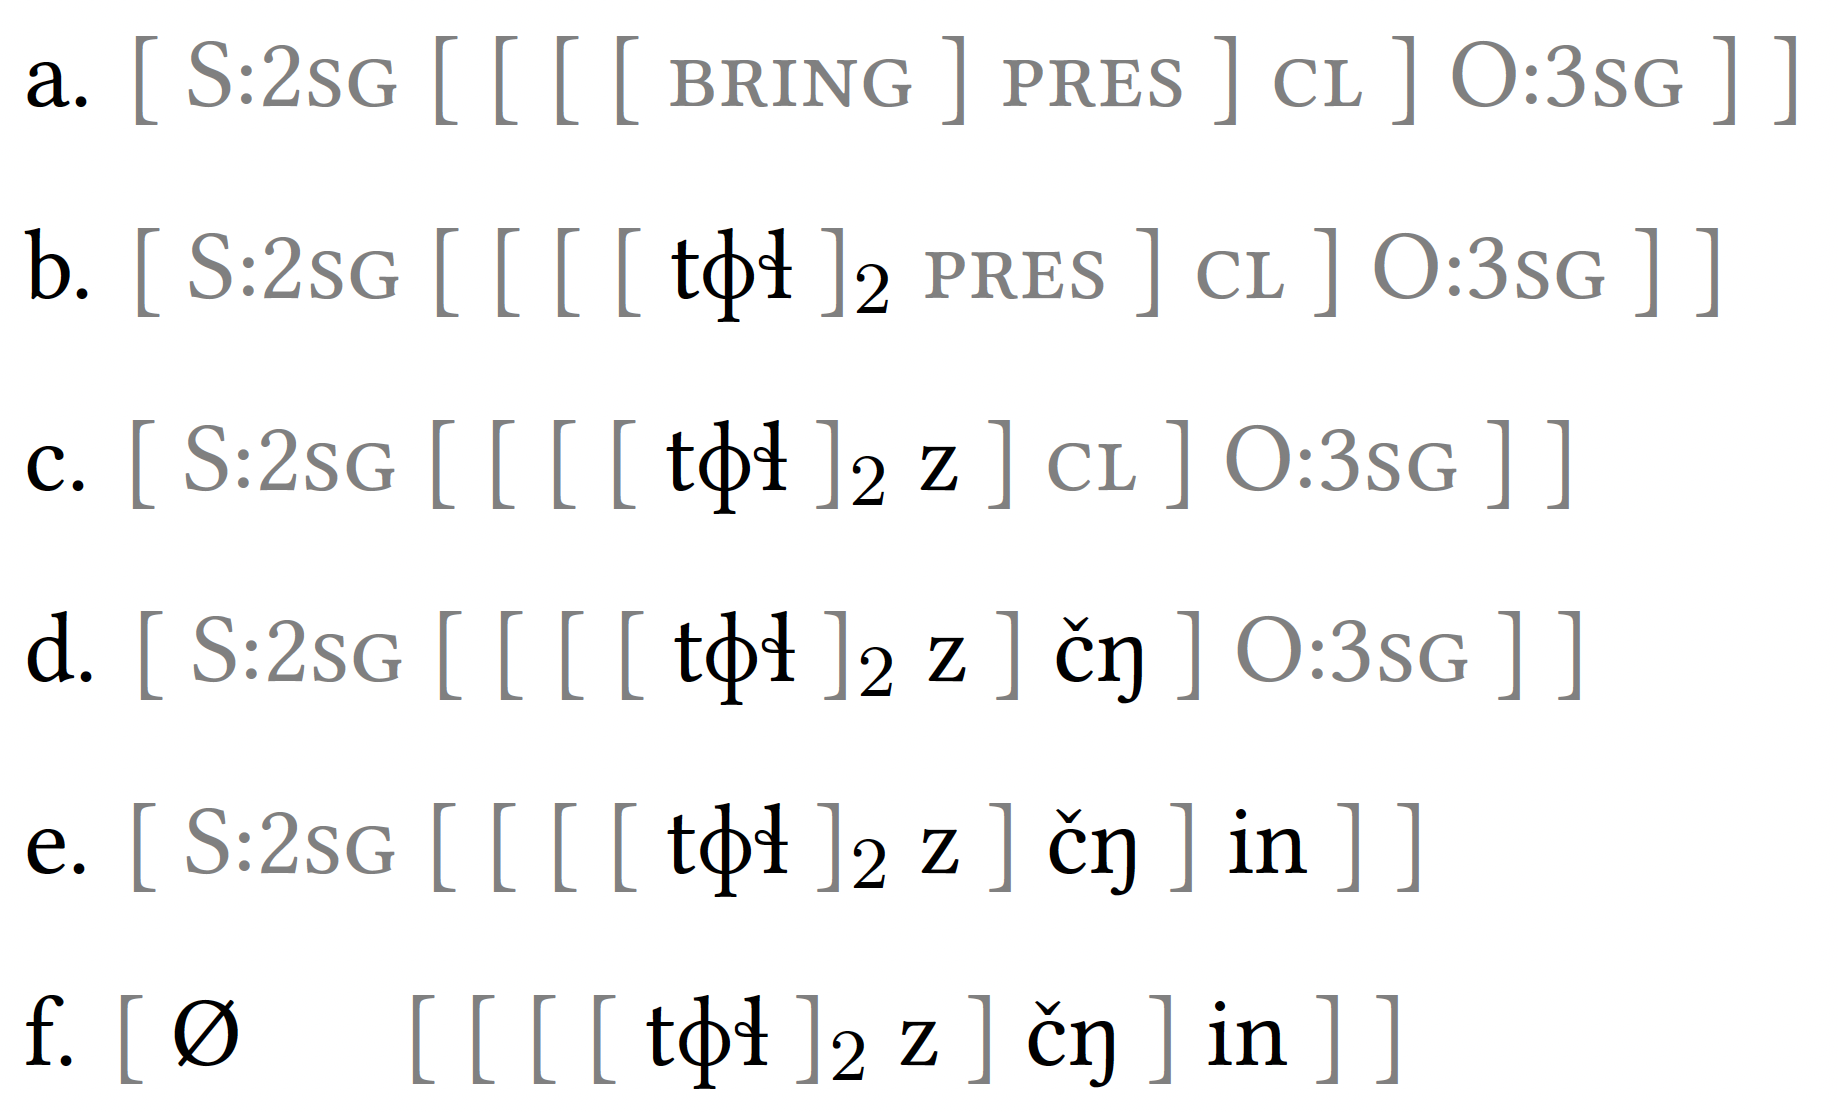
\includegraphics[width=0.5\linewidth]{figs/itelmen.png}

\pex Subject
    \a S:1sg \lra{} t-
    \a S:2 \lra{} \zero{}
\xe
\pex Root
    \a \root{\gsc{bring}} \lra{} tɸɬ
    \a \root{\gsc{embrace}} \lra{} taβol
\xe
\pex Inflection class
    \a cl \lra{} -čŋ / ]2 ] O:3, S:2sg, realis
    \a cl \lra{} -xk / ]2 ] O:[+participant]
    \a cl , -k(i) / ]2
\xe
\pex Object
    \a O:3sg \lra{} -in / ] S:2sg, realis
    \a O:3sg \lra{} -nen / ]S:3
    \a O:3sg \lra{} -čen / ]
\xe

\textbf{Observation:} outward sensitivity to syntactic features (and/or diacritics).

        \subsubsection{Summary}
Allomorphy is sensitive to morphosyntactic triggers that can be either lower (inner) or higher (outer) than the exponent.

Questions (for another time):
    \begin{enumerate} \tightlist
        \item Can any feature be a trigger?
        \item How far away can triggers be? (Locality)
    \end{enumerate}


    \subsection{Phonology: Inward sensitivity}
We've already seen some cases in English, like the past tense and indefinite article (what are some others?).

        \subsubsection{Arabic}
Moroccan Arabic (and other dialects), \cite{rolle21wiley} from \cite{mascaro07} from \cite{harrell62}:
\ex
    \begin{tabular}{l>{\em}ll>{\em}ll}
    a.& xtʕa-h & `his error'  & ktab-u & `his book'\\
    b.& ʃafu-h & `they saw him' & ʃaf-u & `he saw him'\\
    c.& mʕa-h & `with him' & menn-u & `from him'\\
    \end{tabular}
\xe

\bigskip
\pex \gsc{[POSS.3SG.M]} \lra{}
    \a \emph{h} / V \trace{}
    \a \emph{u}
\xe
Issues? Again, doesn't explain the phonotactic logic behind the alternation (historically -\emph{hu}). Remember also that these alternations don't need to be optimizing.
% \ex
%         \begin{tabular}{llll}
%         % Allomorph   &   Environment & Example & Gloss\\ \hline
%         -i  & / C \trace{} & pap-i & `cooked rice'\\
%         -ka & / V \trace{} & ai-ka  & `child'\\
%         \end{tabular}
% \xe

\cite{paster06phd} has more examples of C/V conditioning.

        \subsubsection{Other}
Here's a different natural class, in Tahitian \citep{lazardpeltzer00}:
\ex
    \begin{tabular}{l>{\em}ll>{\em}ll}
    a.& 'amu & `eat' & \textbf{fa'a}-'amu & `make eat'\\
    b.& rave & `do, make' & \textbf{fa'a}-rave & `make make'\\
    c.& tai'o & `read' & \textbf{fa'a}-tai'o & `make read'\\\hline
    d.& mana'o & `think' & \textbf{ha'a}-mana'o & `remember'\\
    e.& fiu & `grow tired' & \textbf{ha'a}-fiu & `be bored'\\
    f.& veve & `be poor' & \textbf{ha'a}-veve & `impoverish'\\
    \end{tabular}
\xe

Here it's labials that condition the form of the affix. They're adjacent on the C tier but not on the segmental tier.

\bigskip
Chaha \citep{jjmcc83}:
\ex Palatalization in the imperative\\
    \begin{tabular}{lll}
    2\gsc{SG.M} & 2\gsc{SG.F} & gloss \\\hline
    nomæd & nomædʲ & `love' \\
    noqo\d{t} & noqo\d{t}ʲ & `kick'\\
    goræz & goræzʲ & `be old'\\
    \end{tabular}
\xe
\ex Labialization in the perfective\\
    \begin{tabular}{lll}
    wihtout object & with object & gloss \\\hline
    qænæf & qænæfʷ & `knock down'\\
    nækæb & nækæbʷ & `find'\\\hline
    nækæs & nækʷæs & `bite' \\
    kæfæt & kæfʷæt & `open' \\\hline
    qæ\d{t}ær & qʷæ\d{t}ær & `kill'\\
    mæsær & mʷæsær & `seem'\\
    \end{tabular}
\xe

Not just the segmental tier but the featural tier! And there's even spreading (in other examples).


\bigskip
Tone-conditioned allomorphy (possessive?) in Mixtepec Mixtex \citep{pastermbeamdeazcona05,paster06phd}: -yù after low tone, otherwise floating L:
\pex Stem ends in H:
    \a vílú + Ⓛ → vílúù 'my cat'
    \a nàmá + Ⓛ → nàmáà 'my soap'
\xe
\pex Stem ends in M:
    \a tzàákū + Ⓛ → tzàákūù 'my coral'
    \a kwà'ā + Ⓛ → kwà'āà 'my sister'
\xe
\pex Stem ends in L:
    \a tūtù + yù → tūtù yù 'my paper'
    \a chá'à + yù → chá'à yù 'I am short'
\xe

\bigskip
Tzeltal perfective depends on the syllable count of the stem \citep{walshdickey99,paster06phd}:
\pex
    \a j-al-\textbf{oh} `he has told something'
    \a s-mah-\textbf{oh} `he has hit something' 
    \a s-kutʃ-\textbf{oh} `she has carried it'
\xe
\pex
    \a s-tikun-\textbf{ɛh} `he has sent something' 
    \a s-mak'lin-\textbf{ɛh} `he has fed someone' 
    \a s-kutʃ-laj-\textbf{ɛh} `she was carrying it repeatedly'
\xe

\bigskip
\cite{rolle21wiley} from \cite{austin81,deakpilbara08}: in Thalanyji, case marking on nouns is sensitive to whether the noun is disyllabic or not. Case marking on pronouns and demonstratives is invariant across both. Except for DAT, whose form is different for each of the three.

See also Western Armenian \citep{dolatian22gjgl}.

\bigskip
\textbf{Observation:} inward sensitivity to phonological material (might be phonologically adjacent in a specific way, like on the C tier).


    \subsection{Phonology: Outward sensitivity}
What would this look like?

\inSolution{
Affix conditions root:
\begin{enumerate}
	\item Root: \emph{pata} `dog'.
	\item With C-initial suffix: \emph{pata-\textbf{k}i} `the dog', \emph{pata-\textbf{m}u} `my dog'.
	\item With V-initial suffix: \emph{\uline{der}-\textbf{a}} `dogs', \emph{\uline{der}-\textbf{e}} `your dog'.
\end{enumerate}
No language like this has been reported! When we find something similar, we also find alternative analyses \citep{adgeretal03tops,kalin20jomo,kastner21li,kiparsky21tlr,dolatian22gjgl}.
}

    \subsection{Theory building}
        \subsubsection{Restrictive theories}

[Exercise]

\paragraph{Phonology} Generative phonology has gone through different formalisms.

What's wrong with this?
\ex /v/ $\rightarrow$ [f] / \trace{} [t]
\xe

\inSolution{
\begin{enumerate} \tightlist
    \item You lose the generalization that this is about voicing.
    \begin{itemize}
        \item There might be a general devoicing/assimilation rule in the language.
    \end{itemize}
    \item You could write anything!
    \ex /g/ $\rightarrow$ [u] / \# \trace{} [n]
    \xe
\end{enumerate}
}

So rule-based phonology concentrated on features from early on \citep{spe}:
\ex {[}+voiced] $\rightarrow$ [--voiced] / \trace{} [--voiced]
\xe

\bigskip
What about that? Well we could still write the following rule using the same formalism:
\ex {[}--voiced] $\rightarrow$ [+voiced] / \trace{} [--voiced]
\xe

And while cases of dissimilation like~(\lastx) are attested, you still lose the generalization that you're either assimilating or dissimilating. So we have alpha-notation:
\ex {[}$\pm$voiced] $\rightarrow$ [$\alpha$ voiced] / \trace{} [$\alpha$ voiced]
\xe

All explicit theories try to account for what's possible and what should be impossible. The strongest ones find ways of building that into the architecture, making strong testable claims.

\paragraph{Syntax} Why was the advent of X-bar theory so important?

Phrase structure grammar:
\pex
    \a S $\rightarrow$ NP VP
    \a NP $\rightarrow$ D (Adj) NP
    \a NP $\rightarrow$ (Adj) N
    \a VP $\rightarrow$ V NP
    \a VP $\rightarrow$ V NP PP
    \a VP $\rightarrow$ \dots{}
    \a PP $\rightarrow$ P NP\\
		\hdashrule[2pt][c]{0.21\linewidth}{1pt}{1.5mm}
    \a V $\rightarrow$ N D VP?
    \a NP $\rightarrow$ \emph{dog} Adv S?
\xe

X-bar theory essentially said:
\pex
    \a XP $\rightarrow$ YP X'
    \a X' $\rightarrow$ X ZP
    \a Figure out what the lexical content of X, Y and Z is in your language.
\xe
So:
\inSolution{
\begin{enumerate} \tightlist
    \item Explains parallels in internal structure of NP, VP, PP, etc.
    \item Predicts head-finality more or less correctly in head-final languages.
\end{enumerate}
}

\paragraph{Semantics} Variables must be bound in their domain. This is why e.g.~donkey sentences are so fascinating to formal semanticists.

\paragraph{Summary} These aren't the only relevant subfields, of course. But:
    \begin{itemize} \tightlist
        \item In each case you're setting up the architecture to tell you both what is and isn't possible.
        \item And then you can think about the origin of that architecture (be it cognitive, historical, etc).
    \end{itemize}

        \subsubsection{A theory of allomorphy}
Let's remind ourselves of what we need to derive (the \emph{explananda}):
\begin{itemize} \tightlist
    \item General distinction between syntactic features and phonological features.
    \item Asymmetry: low material can't see high phonological material (but can see high syntactic material).
    \item Productivity: productive rules exist but so does suppletion.
\end{itemize}

\textbf{What should the architecture look like?} Here are some relevant questions.
\paragraph{Hierarchical relations.} We're assuming a syntactic/morphological/morphosyntactic structure, rather than a linear one (or paradigms, or anything else). Why?
\begin{itemize} \tightlist
    \item Affix order reflects word order.
    \item Words have internal structure so why not.
    \item Inward/outward is not necessarily the same as right/left (though we haven't seen that as such, but we'd expect interactions with syntax).
    \item Uniform module so why not.
\end{itemize}

\paragraph{Late Insertion.} Now let's think about what suppletion teaches us.
\begin{itemize} \tightlist
    \item \emph{Go/went} aren't like \emph{dog$\sim$cat}: one set of syn-sem info is associated with two different forms.
    \item How do you know which form to choose? Depending on the syn and phono information around you.
    \item But when do you know? You can only do that once you have that information.
    \item Lexicalist theories assume that the syntax combines full words. Would that work?
        \begin{itemize} \tightlist
            \item No, because how would you know what word to put at the base of your tree if you don't have the rest of it with the conditioning information yet!
            \item So we need a node to be a bundle of syntax, and only pick the form once you have other nodes with the relevant info around it.
        \end{itemize}
\end{itemize}

\paragraph{Cyclic spell-out.} We still need to understand the contrast between phonological and syntactic conditioning.
\begin{itemize} \tightlist
    \item Where do syntactic and phonological features live in the structure?
    \item How does that relate to Late Insertion?
    \item If you start at the bottom and insert one step at a time, then you can only see the phonological form that's below, not above.
    \item So the different assumptions, when combined, create an architecture which \emph{derives} the generalization.
\end{itemize}

        \subsubsection{Worked example}
Let's think about the alternation \emph{go}$\sim$\emph{went}, and why phonological conditioning can only go in one direction. For simplicity we'll focus on a low node V and a higher node T. I'll use [] for syntactic/semantic features and // for phonological content.

We start, following standard assumptions, by merging the verb or root. At this point, it has some syntactic/semantic features, but we just said it can't have phonology yet, because this root knows it needs to know what tense it is, and T isn't in the structure yet:
\ex \Tree
[.{V\\\root{go}\\syn:[verb]\\phon:/\trace/} ]
\xe

So we go ahead and add T, which by the same logic gives us this:
\ex \label{ex:went-nophono} \Tree
[.
    [.
        [.{V\\\root{go}\\syn:[verb]\\phon:/\trace/} ]    
        [. ]
    ]
    [.{T\\syn:[Past]\\phon:/\trace/} ]
]
\xe

We now have the information that V needs. So we can go ahead and choose its form, or \emph{exponent}, or \emph{vocabulary item}, namely \emph{went}. This is our syntactic conditioning (looking upwards / conditioned downwards):
\ex \Tree
[.
    [.
        [.{V\\\root{go}\\syn:[verb]\\phon:/\textbf{wɛnt}/} ]    
        [. ]
    ]
    [.{T\\syn:[Past]\\phon:/\trace/} ]
]
\xe

Could we have gotten phonological conditioning? Well, at~(\ref{ex:went-nophono}) we didn't have any phonology in T yet. In fact, we always get phonology low (e.g.~in V) before we get it high (e.g.~in T), as this follows from the order in which we derived: we add syntactic objects things bottom-up, and also spell them out bottom-up. If the syntactic features are there first, we're never in a situation in which we have phonology high but not low, like in~(\nextx):
\ex (Does not happen:)\\ \Tree
[.
    [.
        [.{X\\\root{wug}\\syn:[Perf]\\phon:/\trace{}/} ]    
        [. ]
    ]
    [.{Y\\syn:[Past]\\phon:/blɪk/} ]
] 
\xe


        \subsubsection{Summary and readings}
By this point we have more or less built contemporary Distributed Morphology, with some aspects developed most clearly by \cite{embick10}. So see that monograph, or the textbook version in \cite{embick15}.

Embick's system builds on an important paper by Boblajik which focuses on data from Itelmen \citep{bobaljik00}. Those data are reviewed in the excellent overview article of \cite{gouskovabobaljik20cup}. A slightly older overview article is \cite{bonetharbour12}. The textbooks mentioned in the Introduction also deal with allomorphy quite closely.

There are still many questions we haven't explored, such as what the cycles of derivation are like, what the locality relations are, whether there's a difference between suppletion and other kinds of allomorphy, and how else you might deal with any of these issues. Section~\ref{sec:allomorphy:locality} contains additional material on some of these issues, and see also \cite{adgeretal03tops} for a discussion of the architectural issues.

It's also worth mentioning that other theories do have ways of dealing with e.g.~suppletion. Some of the even-stronger evidence for Late Insertion theories comes for patterns of syncretism \citep{kramer20cup}. Other ways of thinking about Late Insertion can be found in \cite{beard95} and \cite{embick16oup}.


    \subsection{Locality} \label{sec:allomorphy:locality}
        \subsubsection{Prelude: \cite{arad03}}
\pex Forms derived from \root{sgr} (after \citealt[746]{arad03}): \label{ex:sgr}
    \a \emph{seger} `closure' (N)
    \a \emph{sograim} `parentheses' (N)
    \a \emph{sgira} `closing' (N)
    \a \emph{sagur} `closed' (A)
    \a \emph{misgeret} `frame' (V)
    \a \emph{sagar} `closed' (V)
    \a \emph{histager} `cocooned himself' (V)
\xe

\bigskip
The verb \emph{misger} `framed' has one consonant ``too many''. \cite{arad03,arad05}: two things persist once you derive the noun.
\begin{itemize} \tightlist
    \item Phonology: The /m/ persists since the verb is derived from the noun \emph{misgeret}, rather than from the root \root{sgr}. 
    \item Semantics: The meaning of `frame' persists in all derived (denominal) forms.
\end{itemize}

\pex
    \a \cmark{} \root{sgr} $\rightarrow$ \emph{misgeret}$_{\text{N}}$ $\rightarrow$ \emph{misger}$_{\text{V}}$
    \a \xmark{} \root{sgr} $\rightarrow$ \emph{misger}$_{\text{V}}$
\xe

\ex \label{ex:kip-trees1}
    a. \Tree 
    [.{v\\\emph{misger}} v [.{n\\\emph{misgeret}} n \root{sgr} ] ]
    \hskip 2cm 
    b. \Tree  [.{n\\\emph{seger}} n \root{sgr} ]
\xe

        \subsubsection{Latin}
Discussion from \cite{embick10,kastnerzu17}.

Latin tree:
\ex \label{tree:latin}
%\begin{small}
\scalebox{0.95}{
a. \Tree
[.TP
    [. ]
    [
        [.T ]
        [.(PerfP)
            [.(Perf) ]
            [.VoiceP
                [.(DP) ]
                [
                    [.Voice ]
                    [.vP
                        [.\root{root} ]
                        [.v ]
                    ]
                ]
            ]
        ]
    ]
]
{\Large $\Rightarrow$}
b. \Tree
[.TP
    [. ]
    [.
        [.PerfP
            [. ]
            [.
                [.VoiceP
                    [.(DP) ]
                    [.
                        [.vP
                            [.\root{root}\\\emph{am}- ]
                            [.v
                                [.v ]
                                [.\gsc{TH}\\-\emph{\=a}- ]
                            ]
                        ]
                        [.\gray{(Voice)} ]
                    ]
                ]
                [.Perf\\-\emph{ve}- ]
            ]
        ]
        [.T 
            [.T{[Fut]}\\-\emph{r}- ]
            [.Agr\\-\emph{\=o} ]
        ]
    ]
]
}
\xe

\paragraph{Perf Conditions T}
The past suffix is usually -\emph{ba}, but is -\emph{(e)ra} when Perf appears.
\pex
    \a  \begingl
        \gla am-\=a-\textbf{ba}-t//
        \glb \root{am}-\gsc{TH}-\textbf{Past}-3\gsc{SG}//
        \glft `he/she loved' \hfill (Default -\emph{ba}-)//
        \endgl
    \a \begingl
        \gla am-\=a-\underline{ve}-\textbf{ra}-t//
        \glb \root{am}-\gsc{TH}-\underline{Perf}-\textbf{Past}-\gsc{3SG}//
        \glft `he/she had loved' \hfill (Special -\emph{ra}-)//
        \endgl
\xe

\paragraph{\fillblank{Root Conditions Perf, Theme Blocks the Conditioning}}\label{sec:latin:analysis:perfroot}
What conditions what?
\pex\label{ex:perf-root}
    \a 
        \begingl
        \gla am-\=a-\textbf{vi}-mus//
        \glb \root{\gsc{LOVE}}-\gsc{TH}-\textbf{Perf}-\gsc{1PL}//
        \glft `we have loved'// % (Default -\emph{v}/\emph{vi}-)//
    \endgl
    
    \a 
        \begingl
        \gla scrip-\textbf{si}-mus//
        \glb \root{\gsc{write}}-\textbf{Perf}-\gsc{1PL}//
        \glft `we have written'// % (Special -\emph{si}-)//
    \endgl
    
    \a 
        \begingl
        \gla v\=en-\textbf{i}-mus//
        \glb \root{\gsc{come}}-\textbf{Perf}-\gsc{1PL}//
        \glft `we have come'// % (Special -\emph{i}-)//
    \endgl
\xe

\begin{answer}{
See \citet[72]{embick10}: Perf conditioned by the root, if the two are adjacent. The theme vowel needs to be null. This pattern is consistent with a locality-based approach if the root and Perf are linearly adjacent.\\
You might know that Latin has conjugation classes, but this is really about the root rather than class: different allomorphs of Perf appear in \emph{men}-\textbf{\emph{u}}-\emph{\={\i}} `I have warned', \emph{aug}-\textbf{\emph{s}}-\emph{\={\i}} `I have increased' and \emph{str\={\i}d}-\textbf{\emph{i}}-\emph{\={\i}} `I have whistled', all second conjugation (Class II).
}\end{answer}

\paragraph{\fillblank{Perf Conditions Agr, T Blocks the Conditioning}}
What conditions what?
\pex \label{ex:perf-agr-pres}
    \a \begingl
        \gla am-\textbf{\=o}//
        \glb \root{am}-\gsc{TH}.\textbf{\gsc{1SG}}//
        \glft `I love'//
    \endgl

    \a \begingl
        \gla am-\=a-\fbox{v}-\textbf{\={\i}}//
        \glb \root{am}-\gsc{TH}-\fbox{Perf}-\textbf{\gsc{1SG}}//
        \glft `I have loved'//
    \endgl
\xe
\pex 
    \a \begingl
        \gla am-\=a-s//
        \glb \root{love}-\gsc{TH}-\gsc{2SG}//
        \glft `you love'//
    \endgl

    \a \begingl
        \gla am-\=a-\fbox{v}-\textbf{isti}//
        \glb \root{love}-\gsc{TH}-\fbox{Perf}-\gsc{2SG}//
        \glft `you have loved'//
    \endgl
\xe

% The \gsc{2SG} ending is usually -\emph{s}, but in the present perfect it is -\emph{ist\={\i}}. The person/number ending of the present is conditioned by linearly adjacent Perf, whereas an overtly realized T blocks the conditioning. With a null T in the present, Perf is linearly adjacent to Agr and can condition contextual allomorphy. When T is overt, as in the past or the future, the default endings appear. 
\begin{answer}{
Agr conditioned by Perf (inward-looking).
}\end{answer}

\bigskip
But we also saw T intervening between Perf and Agr: the 1\gsc{SG} ending for a Class I root like \root{am} `love' is consistent\textemdash \emph{m} in the past and \emph{o} in the future (depending on the value of T).

\pex \label{ex:perf-agr-past2}
    \a \begingl
        \gla am-\=a-\underline{ba}-\textbf{m}//
        \glb \root{am}-\gsc{TH}-\underline{Past}-\textbf{\gsc{1SG}}//
        \glft `I loved'//
    \endgl

    \a \begingl
        \gla am-\=a-\fbox{ve}-\underline{ra}-\textbf{m}//
        \glb \root{am}-\gsc{TH}-\fbox{Perf}-\underline{Past}-\textbf{\gsc{1SG}}//
        \glft `I had loved'//
    \endgl
\xe

\pex \label{ex:perf-agr-fut2}
    \a \begingl
        \gla am-\=a-\underline{b}-\textbf{\=o}//
        \glb \root{am}-\gsc{TH}-\underline{Fut}-\textbf{\gsc{1SG}}//
        \glft `I will love'//
    \endgl

    \a \begingl
        \gla am-\=a-\fbox{ve}-\underline{r}-\textbf{\=o}//
        \glb \root{am}-\gsc{TH}-\fbox{Perf}-\underline{Fut}-\textbf{\gsc{1SG}}//
        \glft `I will have loved'//
    \endgl
\xe

\bigskip
\begin{answer}{
T is closer to Agr, so it gets to condition it. And/or: Agr is conditioned by Perf, but T intervenes.\\
See also \citet[71]{embick10}, \cite{carstairsmccarthy01} and~\cite{adgeretal03tops}.
}\end{answer}

\paragraph{\fillblank{Theme Conditions T, Perf Blocks the Conditioning}}
Traditional grammars: the person endings in the perfect do not change from conjugation to conjugation. What does this mean? Why does it come about?

\bigskip
\begin{answer}{
First, endings usually change from conjugation to conjugation (associated with the theme vowel):
\pex 
    \a \begingl
        \gla am-\underline{\=a}-\textbf{b}-\=o//
        \glb \root{am}-\underline{\gsc{TH}}-Fut-\gsc{1SG}//
        \glft `I will love' (Class I)//
        \endgl
    \a \begingl
        \gla pet-\underline{a}-\textbf{m}//
        \glb \root{pet}-\underline{\gsc{TH}}-Fut.\gsc{1SG}//
        \glft `I will seek' (Class III)//
        \endgl
\xe
\bigskip
What happens in the perfect?
\pex
    \a \begingl
        \gla am-\underline{\=a}-\fbox{ve}-\textbf{r}-o//
        \glb \root{am}-\underline{\gsc{TH}}-\fbox{Perf}-\textbf{Fut}-\gsc{1SG}//
        \glft `I will have loved' (Class I)//
        \endgl
    \a \begingl
        \gla pet-\underline{\=\i}-\fbox{ve}-\textbf{r}-o//
        \glb \root{pet}-\underline{\gsc{TH}}-\fbox{Perf}-\textbf{Fut}-\gsc{1SG}//
        \glft `I will have sought' (Class III)//
        \endgl
\xe
\bigskip
Perf intervenes between TH and T/Agr (and chooses its own allomorph of T).
}\end{answer}

\paragraph{Summary:} Our theory of allomorphy needs to make reference to linear adjacency, which reflects structural adjacency.

        \subsubsection{Nonconcatenative locality: Hebrew}
We'll now test this theory in a domain where we wouldn't expect linear adjacency: nonconcatenative morphology \citep{kastner18nllt,kastner20ogs}.

We need some background and assumptions first.

\paragraph{Background} Semitic verbs come in different ``templates''.

\ex\label{ex:naive-ktb} Some forms for \root{ktb}, generally associated with writing.\\
	\begin{tabular}{lllll}
	& Template & Verb & Gloss & Note\\\hline
	a. & \tkal & katav & `wrote' & unmarked/transitive\\
	b. & \tnif & nixtav & `was written' & anticausative of \tkal~(\ref{ex:naive-ktb}a)\\
	c. & \thif & hextiv & `dictated' & causative of \tkal~(\ref{ex:naive-ktb}a)\\
	d. & \thuf & huxtav & `was dictated' & passive of \thif~(\ref{ex:naive-ktb}c)
	\end{tabular}
\xe
We'll assume that the templates are encoded in Voice, because they reflect argument structure.

\paragraph{Roots}
Some roots change the form of the stem. Assume that the stem vowels are part of the phonology of the template, so are in Voice.
\ex\label{ex:tkal-reg}Some regular roots in \tkal:\\
 \begin{tabular}{llc|ll}
	& \multicolumn{2}{c|}{Root} & Past \gsc{3SG.M} \emph{XaYaZ} & Future \gsc{3SG.M} \emph{jiXYoZ}\\\hline
	a. & `write' & \root{ktb}& katav & jixtov \\
	b. & `wash' & \root{ʃtf}& ʃataf & jiʃtof \\
	c. & `break' & \root{ʃbr} & ʃavar & jiʃbor \\
\end{tabular}
\xe

\ex\label{ex:tkal-irreg}Some irregular roots in {\tkal}:\\
 \begin{tabular}{c|llc|ll|ll}
	Class & & \multicolumn{2}{c|}{Root} & \multicolumn{2}{c|}{Past \gsc{3SG.M}} & \multicolumn{2}{c}{Future \gsc{3SG.M}}\\\hline
	\multirow{2}{*}{/j/-final \root{XYj}}
		& a. & `happen' & \root{\dgs{k}rj}& kar\uline{a}&(*kara\uline{j}) & jikr\uline{e} & (*jikroj) \\
		& b. & `want' & \root{r\texttslig{}j}& ra\texttslig{}\uline{a}&(*ra\texttslig{}a\uline{j}) & jir\texttslig{}\uline{e} & (*jir\texttslig{}oj) \\\hline
	\multirow{1}{*}{/ʔ/-final \root{XYʔ}}
		& c. & `freeze' & \root{\dgs{k}pʔ}& kaf\uline{a}&(*kafa\uline{ʔ}) & jikp\uline{a} & (*jikpoʔ) \\\hline
	\multirow{3}{*}{/n/-initial \root{nYZ}}
		& d. & `fall' & \root{npl}& nafal& & j\uline{ip}ol & (*jinpol) \\
		& e. & `give' & \root{ntn}& natan& & j\uline{i}t\uline{e}n & (*jinton) \\
		& f. & `avenge' & \root{n\dgs{k}m}& nakam& & ji\uline{n}kom &  \\
\end{tabular}
\xe

Similar effects arise in other templates, for instance in~\tpie~in~(\nextx).
\ex\label{ex:tpie-irreg}A regular and irregular root in \tpie:\\
 \begin{tabular}{c|llc|l|l}
	Class & & \multicolumn{2}{c|}{Root} & Past \gsc{3SG.M} & Future \gsc{3SG.M}\\\hline
	Regular \root{XYZ}
		& a. & `complicate' & \root{sbx}& sibex & jesabex  \\
	Doubled \root{XYY}
		& b. & `spin' & \root{svv}& s\uline{o}vev & jes\uline{ov}ev  \\
\end{tabular}
\xe

Voice is conditioned by Root:
\ex
\Tree
    [.TP
        [.\tikz{\node (TAgr) {T+Agr};} ]
        [
            [.\tikz{\node (Voice) {Voice};} ]
            [
                [.v\\{(covert)} ]
                [.\tikz{\node (Root) {\root{root}};} ]
            ]
        ]
    ]
\begin{tikzpicture}[overlay]
    \draw[dotted,thick,->] (Root) .. controls +(south:1) and +(south:2) .. (Voice);
\end{tikzpicture}
\xe

\paragraph{T and Voice} Let's look at the stem vowels in a few paradigms (two different templates).
\ex \label{ex:1st2nd}
	\begin{tabular}{l|ll}
		 & \multicolumn{2}{c}{\emph{hegdil} `enlarged'}\\
		 & \gsc{SG} & \gsc{PL}\\	\hline
		\red{1} & hegd\textbf{\green{a}}l-\blue{t}i & hegd\textbf{\green{a}}l-\blue{n}u\\
		\red{2\gsc{M}} & hegd\textbf{\green{a}}l-\blue{t}a & hegd\textbf{\green{a}}l-\blue{t}em\\
		\red{2\gsc{F}} & hegd\textbf{\green{a}}l-\blue{t} & hegd\textbf{\green{a}}l-\blue{t}em\\\hline
		3\gsc{M} & hegd\textbf{i}l-\zero{} & hegd\textbf{i}l-u\\
		3\gsc{F} & hegd\textbf{i}l-a & hegd\textbf{i}l-u
	\end{tabular} \hfil
	\begin{tabular}{l|ll}
	 & \multicolumn{2}{c}{\emph{gidel} `grew'}\\
	 & \gsc{SG} & \gsc{PL}\\	\hline
		\red{1} & gid\textbf{\green{a}}l-\blue{t}i & gid\textbf{\green{a}}l-\blue{n}u\\
		\red{2\gsc{M}} & gid\textbf{\green{a}}l-\blue{t}a & gid\textbf{\green{a}}l-\blue{t}em\\
		\red{2\gsc{F}} & gid\textbf{\green{a}}l-\blue{t} & gid\textbf{\green{a}}l-\blue{t}em\\\hline
		3\gsc{M} & gid\textbf{e}l-\zero{} & gid\sout{\textbf{\gray{e}}}l-u\\
		3\gsc{F} & gid\sout{\textbf{\gray{e}}}l-a & gid\sout{\textbf{\gray{e}}}l-u
	\end{tabular}
\xe

\bigskip
The stem vowel depends on the subject's person value.

\pex \label{tree:locality1}
\Tree
    [.TP
        [.\tikz{\node (TAgr) {T+Agr};} ]
        [
            [.\tikz{\node (Voice) {Voice};} ]
            [
                [.v\\(covert) ]
                [.\tikz{\node (Root) {\root{root}};} ]
            ]
        ]
    ]
    \begin{tikzpicture}[overlay]
    %\draw[semithick,->] (TAgr) to[out=south west,in=south west] (Voice);
    \draw[dotted,thick,->] (Root) .. controls +(south:1) and +(south:2) .. (Voice);
    %\draw[dotted,thick,->] (TAgr) to[out=225,in=270] (Voice);
    \draw[dotted,thick,->] (TAgr) .. controls +(south west:1) and +(south west:1) .. (Voice);
    \end{tikzpicture}
\xe

\paragraph{Prediction: Root and T+Agr}
What might we predict next about the interaction of Root, Voice and T+Agr?

\begin{enumerate} \tightlist
    \item Root and Voice: linearly adjacent. Already seen that Root conditions Voice.
    \item Voice and T+Agr: linearly adjacent. Different agreement affixes depending on the template. This is correct.
    \item Root and T+Agr: overt Voice intervenes. The same agreement affixes are used regardless of root class. This is correct.
\end{enumerate}

\ex\label{tree:locality2}
\Tree
    [.TP
        [.\tikz{\node (TAgr) {T+Agr};} ]
        [
            [.\tikz{\node (Voice) {Voice};} ]
            [
                [.{v\\(covert)} ]
                [.\tikz{\node (Root) {\root{root}};} ]
            ]
        ]
    ]
    \begin{tikzpicture}[overlay]
    \draw[dotted,thick,->] (TAgr) .. controls +(north west:2) and +(north east:2) .. (TAgr);
    \draw[dotted,thick,->] (Voice) .. controls +(south:1) and +(south:1) .. (TAgr);
    \draw[dotted,thick,->,red] (Root) .. controls +(south:2) and +(south west:2) .. node{\large $\times$}(TAgr);
	\end{tikzpicture}
\xe

\bigskip
\paragraph{Prediction: Passives}
What would happen if we now have something between Voice and T+Agr? Enter the passive!

The difference we saw in~(\ref{ex:1st2nd}) no longer exists, here for \emph{biʃel} `cooked':
\ex
	\begin{tabular}{ll|ll}
	& Template & Past \gsc{3SG.M} & Past \gsc{1SG} \\\hline
	a.& \tpie~(active)  & bi\textipa{S}\underline{\'e}l & bi\textipa{S}\underline{\'a}l-ti \\
	b.& \tpua~(passive) & b\textbf{u}\textipa{S}\textbf{\underline{\'a}}l & b\textbf{u}\textipa{S}\textbf{\underline{\'a}}l-ti \\
	\end{tabular}
\xe

\bigskip
Tense doesn't matter either: there might be a difference in vowels between past and future in the active,~(\nextx a), but not in the passive,~(\nextx b).
\ex 
	\begin{tabular}{ll|ll}
	& Template & Past \gsc{3SG.M} & Future \gsc{3SG.M} \\\hline
	a.& \tpie~(active)  & b\underline{i}\textipa{S}\'el & je-v\underline{a}\textipa{S}\'el \\
	b.& \tpua~(passive) & b\textbf{\underline{u}}\textipa{S}\textbf{\'a}l & je-v\textbf{\underline{u}}\textipa{S}\textbf{\'a}l \\
	\end{tabular}
\xe

\bigskip
\textbf{Generalization:} The stem vowels are always \emph{-u-a-} in the passive.

Full paradigms:
\pex\label{table:pass-vowels}
%\a Past tense for passive \emph{pukad} `was commanded' and \emph{hufkad} `was deposited':\\
\a Past of passive \emph{gudal} `was raised' and \emph{hugdal} `was enlarged':\\
\begin{tabular}{l||ll|ll}
 & \multicolumn{2}{c}{\tpua~\root{gdl}}	& \multicolumn{2}{c}{\thuf~\root{gdl}}\\
 & \gsc{SG} & \gsc{PL}	& \gsc{SG} & \gsc{PL}\\\hline
1 & g\textbf{u}d\textbf{\'a}l-ti & g\textbf{u}d\textbf{\'a}l-nu		& h\textbf{u}gd\textbf{\'a}l-ti & h\textbf{u}gd\textbf{\'a}l-nu\\
2M & g\textbf{u}d\textbf{\'a}l-ta & g\textbf{u}d\textbf{\'a}l-tem	& h\textbf{u}gd\textbf{\'a}l-ta & h\textbf{u}gd\textbf{\'a}l-tem\\
2F & g\textbf{u}d\textbf{\'a}l-t & g\textbf{u}d\textbf{\'a}l-tem	& h\textbf{u}gd\textbf{\'a}l-t & h\textbf{u}gd\textbf{\'a}l-tem\\
3M & g\textbf{u}d\textbf{\'a}l & g\textbf{u}d\del{\textbf{\'a}}l-{\'u}	& h\textbf{u}gd\textbf{\'a}l & h\textbf{u}gd\del{\textbf{\'a}}el-{\'u}\\
3F & g\textbf{u}d\del{\textbf{\'a}}l-{\'a} & g\textbf{u}d\del{\textbf{\'a}}l-{\'u}	& h\textbf{u}gd\del{\textbf{\'a}}el-{\'a} & h\textbf{u}gd\del{\textbf{\'a}}el-{\'u}
\end{tabular}

\a Future of passive \emph{jegudal} `will be raised' and \emph{jugdal} `will be enlarged':\\
%\a Future tense for passive \emph{jefukad} `will be commanded' and \emph{jufkad} `will be deposited':\\
\begin{tabular}{l||ll|ll}
 & \multicolumn{2}{c}{\tpua~\root{gdl}}	& \multicolumn{2}{c}{\thuf~\root{gdl}}\\
 & \gsc{SG} & \gsc{PL}	& \gsc{SG} & \gsc{PL}\\\hline
1 & j-e-g\textbf{u}d\textbf{\'a}l & n-e-g\textbf{u}d\textbf{\'a}l		& j-\textbf{u}gd\textbf{\'a}l & n-\textbf{u}gd\textbf{\'a}l\\
2M & t-e-g\textbf{u}d\textbf{\'a}l & t-e-g\textbf{u}d\del{\textbf{\'a}}l-{\'u}	& t-\textbf{u}gd\textbf{\'a}l & t-\textbf{u}gd\del{\textbf{\'a}}el-{\'u}\\
2F & t-e-g\textbf{u}d\del{\textbf{\'a}}l-{\'i} & t-e-g\textbf{u}d\del{\textbf{\'a}}l-{\'u}	& t-\textbf{u}gd\del{\textbf{\'a}}el-{\'i} & t-\textbf{u}gd\del{\textbf{\'a}}el-{\'u}\\
3M & j-e-g\textbf{u}d\textbf{\'a}l & j-e-g\textbf{u}d\del{\textbf{\'a}}l-{\'u}	& j-\textbf{u}gd\textbf{\'a}l & j-\textbf{u}gd\del{\textbf{\'a}}el-{\'u}\\
3F & t-e-g\textbf{u}d\textbf{\'a}l & j-e-g\textbf{u}d\del{\textbf{\'a}}l-{\'u}	& t-\textbf{u}gd\textbf{\'a}l & j-\textbf{u}gd\del{\textbf{\'a}}el-{\'u}
\end{tabular}
\xe

\bigskip
And this is exactly what we'd expect:
\ex\label{tree:locality3}
\Tree
    [.TP
        [.\tikz{\node (TAgr) {T+Agr};} ]
        [
	        [.\textbf{Pass}\\{\tikz{\node (Pass) {\textbf{\emph{u}}};}} ]
	        [
	            [.Voice\\{\tikz{\node (Voice) {\emph{\textcolor{red}{he,a}}};}} ]
	            [
	                [.v\\{(covert)} ]
	                [.\tikz{\node (Root) {\root{root}};} ]
	            ]
	        ]
        ]
    ]
    \begin{tikzpicture}[overlay]
    \draw[dotted,thick,->] (TAgr) .. controls +(north west:2) and +(north east:2) .. (TAgr);
    \draw[dotted,thick,->,red] (TAgr) .. controls +(south west:3) and +(south west:2) .. node{\large $\times$}(Voice);
    \draw[dotted,thick,->] (Voice) .. controls +(south:1) and +(south:2) .. node{\large $\times$}(TAgr);
    \draw[dotted,thick,->] (Root) .. controls +(south:2) and +(south west:3) .. node{\large $\times$}(TAgr);
    \end{tikzpicture}
\xe





    \subsubsection{Cyclicity: French prepositions and determiners}
\paragraph{D-N cliticization.}
\citet[87]{embick10}: adjoin D to vowel-initial nouns when adjacent.
\pex
    \a \emph{le chat} `the cat' (M)
    \a \emph{la mère} `the mother' (F)
\xe
\pex
    \a \emph{l'arbre} `the tree' (M), *\emph{le arbre}
    \a \emph{l'abeille} `the bee' (F), *\emph{la abeille}
\xe

\ex
\Tree
    [.DP
        [. ]
        [.
            [.D ]
            [.NP [.{N\\\emph{C-/V-}} ] ]
        ]
    ]
\xe
So you need some allomorphy-like rule for D and N (which are almost always adjacent), which cares about the phonology of inner N.

\paragraph{P-D fusion.} Some prepositions ``fuse'' with the definite article: \emph{de} `of' and \emph{à} `to' in the masculine, plus \emph{à} in the feminine plural:
\ex
    \begin{tabular}{l>{\em}l>{\em}ll}
        & \normalfont{``Fused''} & \normalfont{Separate} & gloss\\\hline
    \multirow{3}{*}{Masc} & du chat  & *de le chat   & `of the cat'\\
        & au chat   & *à le chat    & `to the cat'\\
        & aux chats & *à les chats  & `to the cats'\\\hline
    \multirow{3}{*}{Fem} & * & de la mère    & `of the mother'\\
        & * & à la mère & `to the mother'\\
        & aux mères & *à les mères & `to the mothers'\\
    \end{tabular}
\xe

\ex
\Tree
[.PP
    [.P ]
    [.DP
        [. ]
        [.
            [.D ]
            [.NP [.{N\\\emph{C-/V-}} ] ]
        ]
    ]
]
\xe
So we need a rule which combines P and D, depending on their syntactic features/diacritics.

\paragraph{Cyclicity.} What would be a situation in which either rule could apply?

With a V-initial noun, e.g.~\emph{de} + \emph{le} + \emph{arbre} `of the tree'? One rule applies to P+D and the other to D+N. What are the predictions in each case?

\begin{answer}{
\ex
\Tree
[.PP
    [.{P\\\emph{de}} ]
    [.DP
        [. ]
        [.
            [.{D\\\emph{le}} ]
            [.NP [.{N\\\emph{arbre}} ] ]
        ]
    ]
]
\xe
\bigskip
What we actually find is no fusion:
\pex \a \emph{de l'arbre}
    \a \ljudge{*} \emph{du arbre}
\xe
\bigskip
Why no fusion? Because you first adjoin D to N. This makes sense if \textbf{the derivation proceeds cyclically, from the bottom up}.
}\end{answer}
% stopped at p. 92 of his book


\paragraph{Locality conditions.} As \cite{gouskovabobaljik20cup} mention, locality in allomorphy might be weaker than strict adjacency. See for instance \cite{kastnermoskal18}, \cite{merchant15li}, \cite{christopoulospetrosino18} and \cite{sandeetal20}.


    \subsection{Discussion: Allomorphy and allosemy across domains}
We've ended up with a cyclic, modular, bottom-up, local theory of allomorphy. Along the way we've assumed that syntax and morphology can be the same module, and Late Insertion of phonological material.

Now recall: what did \cite{arad03} conclude about how meaning is computed across derivations based on Hebrew?

Combining Arad's proposal with the locality conditions on allomorphy, \cite{marantz13} argues for similar locality conditions for allomorphy and meaning. This is an architectural point: the structure (syntax/morphology) imposes constraints on how each module (phonology, morphology) gets its own information.

\bigskip
Combining the unpredictable meaning with special allomorphy for English nouns \citep{embick10}:
\ex[exno=31]
    \begin{tabular}{>{\em}l>{\em}l}
    refus-al & refus-ing\\
    marri-age & marry-ing\\
    destruct-ion & destruct-ing\\\hline
    dance-\zero{} & danc-ing\\
    break-Ø & break-ing\\\hline
    curios-ity & curious-ness\\
    \end{tabular}
\xe

\bigskip
One possible (Arad-style) analysis:
\ex
    a. \Tree 
    [.{n\\\emph{refusal}}
        [.\root{\gsc{refuse}} ]
        [.{n\\\emph{-al}} ]
    ]
    \hspace{2cm}
    b. \Tree
    [.{n\\\emph{refusing}} 
        [.v
            [.\root{\gsc{refuse}} ]
            [.{v\\\zero{}} ]
        ]
        [.{n\\\emph{-ing}} ]
    ]
\xe

See \cite{kastner19cup} for an overview of this last bit.

\paragraph{Further reading: *ABA.} \cite{bobaljik12}, \cite{smithetal16supplet}, \cite{mueller20}, and the articles in \cite{cahavanden17}.


% \newpage

%     \subsection*{Bonus: Hungarian (material incomplete)}
% Hungarian (also \citealt{tabachnik21dp}):

% Plural is -(V)\emph{k} (depends on the stem, plus there's vowel harmony):
% \pex 
%     \a csont-ok\\
%     `bones'
%     \a fog-ak\\
%     `teeth'
% \xe

% Possession is marked on the possessed item:
% \pex
%     \a \begingl
%         \gla az (\H{o}) csont -ja -Ø//
%         \glb the her bone -\gsc{poss} -\gsc{3sg}//
%         \glft `her bone'//
%     \endgl
%     \a \begingl
%         \gla az (\H{o}) fog -a -Ø//
%         \glb the her tooth -\gsc{poss} -\gsc{3sg}//
%         \glft `her tooth'//
%     \endgl
% \xe

% \ex[exno=62] Hungarian plural possessive \citep[165]{carstairs87}\\
%     \begin{tabular}{llllll}
%     & \gsc{sg}  & \gsc{sg}, \gsc{1sg.poss}    & \gsc{pl}  & \gsc{pl}, \gsc{1sg.poss} & Gloss\\\hline
%     a.& ruha & ruhá-m & ruhá-k & ruha-ái-m & `(my) dress(es)'\\
%     b.& kalap & kalap-op & kalap-ok & kalap-jai-m & `(my) hat(s)'\\
%     c.& ház & ház-am & ház-ak & ház-ai-m & `(my) house(s)'\\
%     \end{tabular}
% \xe

% From \cite{rolle21wiley}:
% \ex \cite{carstairsmccarthy01}\\
%     \begin{tabular}{llll}
%     & \gsc{SG} & \gsc{PL} & \\
%     a.& dal & dal-o-k & `song'\\\hline
%     b.& dal-o-m & dal-a-i-m & `my song(s)'\\
%     c.& dal-o-d & dal-a-i-d & `your.\gsc{SG} song(s)'\\
%     d.& dal-a-Ø & dal-a-i-Ø & `his/her song(s)'\\
%     e.& dal-u-nk & dal-a-i-nk & `our song(s)'\\
%     f.& dal-o-tok & dal-a-i-tok & `your.\gsc{PL} song(s)'\\
%     g.& dal-u-k & dal-a-i-k & `their song(s)'\\
%     \end{tabular}
% \xe


% \ex \begingl
%     \gla az (\H{o}) csont -ja \textbf{-i} -Ø//
%     \glb the her bone -\gsc{poss} -\gsc{PL} -\gsc{3sg}//
%     \glft `her bones'//
%     \endgl
% \xe

% Possessor agreement:
% \pex 
%     \a \begingl
%     \gla az (én) csont -Ø -om//
%     \glb the my bone -\gsc{poss} -\gsc{1sg}//
%     \glft `my bone'//
%     \endgl

%     \a \begingl
%     \gla az (én) csont -ja \textbf{-i} -m//
%     \glb the her bone -\gsc{poss} -\gsc{PL} -\gsc{1sg}//
%     \glft `her bones'//
%     \endgl
% \xe

% \pex
%     \a \gsc{pl} \lra{} -((j)a)i- / \trace{} \gsc{Poss}
%     \a \gsc{pl} \lra{} -(V)k
%     \a \gsc{Agr[1sg]} \lra{} -m
% \xe



% \section{*ABA (incomplete)}

%     \subsection{Comparatives and superlatives}
    
%     \subsection{Extending to inchoatives}
    
%     \subsection{Extending to case and pronouns}
% Smith et al

%     \subsection{More}
% McFadden, \cite{mueller20}, Andersson.


% \newpage

\section*{Interim recap}

We started off this course by considering the different things morphology interacts with. In order to start somewhere, we concentrated on cases where morphemes interact with one another:

\ex \Tree
    [.{Morpheme-to-morpheme interactions}
        [.{Affix ordering\\ (\emph{morphotactics})} ]
        [.{Morphophonology\\(\emph{allomorphy})} ]
    ]
\xe

We saw that:
\begin{enumerate} \tightlist
    \item We can make sense of affix ordering if we think of morphological structure in terms of syntactic-semantic structure.
    \item There are independent reasons to think that there is hierarchical structure in morphology (ambiguity, etc).
    \item A specific view of syntactic structure plus phonological Late Insertion predicts crosslinguistic patterns of allomorphy.
\end{enumerate}

This kind of theory is inspired by Distributed Morphology but is consistent with a number of other related frameworks, including the Exo-Skeletal Model \citep{borer05vol1,borer05vol2,borer13oup,borer14lingua,acedomatellanmateu14}, First Phase Syntax \citep{ramchand08} and Nanosyntax \citep{caha16dm}.

Now it's time to see how explanatory this kind of theory is. We will look at the interaction of morphology and syntax (argument structure), followed by the interaction of morphology and semantics (lexical semantics).

\section{Argument structure}

	\subsection{Preliminaries}
	    \subsubsection{Valency}
Verbs differ in terms of the number of syntactic and semantic dependents they require (or are compatible with). This is often called verb valency.

\ex It rained.
\xe
\pex
	\a Chris ran.
	\a The door opened.
\xe
\pex
	\a Chris hit the ball.
	\a Chris knows the answer.
\xe
\pex
	\a Sam put the book on the table.
	\a \ljudge{*} Sam put the book.
	\a \ljudge{*} Sam put on the table.
	\a Sam gave Tyler a book.
	\a \ljudge{*} Sam gave Tyler.
	\a \ljudge{*} Sam gave a book.
\xe

\textbf{Observation:} \fillblank{Verbs (in English) require at most one \textbf{external} argument, one \textbf{internal} argument and one \textbf{indirect/applied/oblique} argument at the same time.}

\bigskip
Do any verbs take more than 3 dependents (subject plus two objects)?

\begin{answer}{
Transactional verbs seem to imply 3 complements semantically but don’t require that all be expressed:
\pex
    \a Max bet Sam (£20) (that he would win the race).
    \a Itamar bought a house (from Michael) (for £40).
\xe
}\end{answer}

        \subsubsection{External arguments}
Let's look at \emph{external arguments} (subjects) more closely. In~(\nextx)--(\anextx) we see cases where the external argument (subject) varies but the verb and internal argument (object) stay the same. How do the readings within~(\nextx) and within~(\anextx) differ?

\pex
	\a Kim took a nap.
	\a The child took a nap.
	\a The dog took a nap.
	\a \ljudge{?} The computer took a nap.
\xe

\pex 
	\a Kim threw the ball.
	\a The child threw the ball.
	\a The monkey threw (the dog) the ball.
\xe

\bigskip

\begin{answer}{
It's the same event, except with a different subject/agent. Even the computer example makes sense if we think of the ``sleep'' function.
}\end{answer}

\bigskip

Now, in~(\nextx)--(\anextx), we see cases where the internal argument varies while the verb and external argument stay the same. How do the readings differ within~(\nextx) and~(\anextx)? How are these cases different from those in~(\blastx)--(\lastx)?

\pex
	\a Kim took a nap.
	\a Kim took a book from the shelf.
	\a Kim took a bus.
\xe

\pex
	\a Kim threw the ball.
	\a Kim threw a party.
	\a Kim threw a tantrum.
	\a Kim threw the match [lost it on purpose].
\xe

\begin{answer}{
The kind of event changes, depending on the object, even though the verb stays the same. And in all cases we still have an internal argument (object), so the syntax stays more or less the same.
}\end{answer}

\bigskip
\paragraph{Generalization.} \fillblank{The semantic relationship between the verb and the internal argument is less predictable than that between the verb and the external argument, which is predictable.}

How can we derive this generalization in our formal system?

\begin{itemize} \tightlist
    \item \fillblank{It appears that a predicate has selectional requirements for its complement, but less so for its subject.}
    \item \fillblank{This makes sense if the verb and internal argument form one domain (much like a root and the first categorizing affix), with the external argument being added later in the derivation.}
    \item \fillblank{One common way of doing this technically is by using a separate head to introduce the external argument. For \cite{chomsky95} this is ``little \emph{v}''. Other work since calls this head Voice \citep{kratzer96,marantz97,marantz13lingua,pylkkanen08,layering15,kastner20ogs}.}
\end{itemize}

Tree:
\ex \emph{Sam ate cake}:\\
\Tree
[.TP
	\qroof{\tikz{\node (SpecTP) {\emph{Sam}};}}.DP
	[.T'
		[.T[Past] ]
		[.VoiceP
			\qroof{\tikz{\node (SpecVoice) {\emph{\sout{Sam}}};}}.DP
			[.
				[.Voice ]
				[.vP
					[.{v\\\emph{ate}}
						[.\root{\gsc{EAT}} ]
						[.v ]
					]
					\qroof{\emph{cake}}.DP
				]
			]
		]
	]
]
\begin{tikzpicture}[overlay]
	\draw[thick,->] (SpecVoice) .. controls +(south west:2) and +(south west:2) .. node[below]{\scriptsize (EPP)\phantom{aa}}(SpecTP);
\end{tikzpicture}
\xe
\bigskip

See \cite{kratzer96} for the original proposal; the paper gets a bit technical at times but is fairly readable overall. See chapter 1.3 of \cite{layering15} or chapter 1.3.1 of \cite{kastner20ogs} for a very quick overview.

    \subsection{Sublexical modification}
Now let's go deeper into argument structure by seeing how morphology and syntax interact.
        
        \subsubsection{Syntax}

What are the possible readings for~(\nextx)?
\ex Itamar turned the wi-fi off again.
\xe

\bigskip
\begin{answer}{
\pex \a The new router arrived from the factory. The tech people plugged it in, turned it on, and then Itamar turned it back off. \hfill [\emph{restitutive}]
	\a Alex turned the wi-fi off so that students would focus on his lecture. At the end of the lecture he turned it back on. Then Itamar turned it off again for his own lecture. \hfill [\emph{repetitive}]
	\a Before every lecture, Itamar turns the wi-fi off so that students focus on his lecture. He'd done so for the past six weeks, and has just turned it off again. \hfill [\emph{repetitive}]
\xe
\emph{Again} can modify either being-off (restitutive, a), or causing-something (repetitive, b--c).
}\end{answer}

\bigskip
We can do this with various predicates:
\ex Chris opened the door again.
\xe

\begin{answer}{
\pex \a The door had been open before. Maybe it was built open, then someone closed it, then Chris opened it. \hfill [\emph{restitutive}]
	\a Someone else opened the door, someone closed the door, and then Chris opened the door. \hfill [\emph{repetitive}]
	\a Chris had already opened the door once, then they opened it a second time. \hfill [\emph{repetitive}]
\xe
\emph{Again} can modify either becoming-open (restitutive, a), or causing-something (repetitive, b--c).
}\end{answer}

\bigskip
How do we capture this formally? Say we schematize an event the following way \citep{vonstechow96,beckjohnson04,dowty91}. What can \emph{again} modify?

\ex {[}Chris CAUSE [door BECOME open]]
\xe

\begin{answer}{
If \emph{again} modifies BECOME, we get the restitutive reading. If it modifies CAUSE, we get the repetitive reading.\\
Or in a tree: 
\citep{kratzer96,dm,layering15,kastner20ogs}
\ex
\Tree
	[.VoiceP
		[.\emph{Chris} ]
		[.
			[.Voice ]
			[.vP 
				[.v 
					[.\root{open} ]
					[.v ]
				]
				[.{DP\\\emph{the door}} ]
			]
		]
	]
\xe
\pex In such a structure, \emph{again} could adjoin to (and modify):
	\a The root \root{open} (restitutive).
	\a The vP, perhaps together with Voice (repetitive, `someone' reading).
    \a The full VoiceP (repetitive, `Chris' reading).
\xe
We can imagine various analytical choices. Does \emph{again} attach to different parts of the tree in the syntax? Or does it attach in one set place, but then combine with different constituents in the semantics?
}\end{answer}

\bigskip
One prediction of this view is that \emph{again} shouldn't be able to modify only part of a constituent. For example, we wouldn't expect \emph{again} to modify the entire VoiceP but without the internal argument. In other words, the following reading should not be possible - which is correct:
\ex Itamar turns the air conditioning off before each class. But today he flipped the wrong switch. Today, \# Itamar turned the WI-FI off again.
\xe

        \subsubsection{Morphology}
Is there an affix that does the same job as \emph{again}, and has the same readings?

\ex \fillblank{Chris \textbf{re-}opened the door.}
\xe

\bigskip

Other affixes influence argument structure. How?

\pex \a  I danced.
	\a \ljudge{*} I danced Eryl.
\xe
\pex \a \ljudge{*} I out-danced.
	\a I out-danced Eryl.
\xe

The following verbs seem to allow \emph{out}-prefixation easily:
\pex \a swim, dance, jump, eat.
	\a I out-swam/out-danced/out-jumped/out-ate Eryl.
\xe

But these ones resist it (at least with the meanings they have when used with just a subject and no object).
\pex \a appear, arrive, die.
	\a \judge{*} I out-appeared/out-arrived/out-died Eryl.
\xe

What's the difference between the verbs that allow it and the ones that don't?

\begin{answer}{
In English, \emph{out}-prefixation attaches to verbs that don't \emph{need} an object, and creates a standard of comparison out of the new object.\\
See \cite{ahn22}.
}\end{answer}

\bigskip
And do the following sentences change our description of the behavior of \emph{out}-prefixation?
\pex 
    \a \ljudge{*} The bus ran
	\a I out-ran the bus.
    \a \ljudge{*} My pajamas grew
    \a I out-grew my pajamas.
\xe


\bigskip
Here's a similar example, Spanish \emph{sobre}- `over' \citep[100]{fabregasscalise12}:

\pex
    \a \begingl
        \gla El pájaro vuela.//
        \glft `The bird flies.'//
    \endgl
    \a \begingl
        \gla El pájaro sobrevuela *(la casa)//
        \glb The bird over-flies (the house)//
        \glft `The bird flies over the house.'//
    \endgl
\xe

\bigskip
\textbf{Summary.} Events, or verb phrases in technical terms, have internal structure. We can isolate parts of this structure through \emph{sublexical modification}: modifying part of an opening event, for example, using an adverbial. See chapter 2.2.2.1 of \cite{layering15} for more on this.

If syntax and morphology are the same module, we expect that these adverbials could be either words or affixes - as is the case. And these elements which we add can also change the argument structure of the verb (adding or removing arguments), in ways which we haven't made precise yet.

    \subsection{Causativization}
        \subsubsection{Thinking structurally}
[Jigsaw puzzle: how do we express causation? What are some of the kinds of \emph{causative verbs} that we find?]

% What do we think is going on in each case?
% \pex
%     \a Destroy the tower. (transitive/causative)
%     \a Open the door. (labile/alternating)
%     \a Make Sam dance. (periphrastic)
% \xe

We have seen examples of:
\pex
    \a ``Lexical'' causatives, where the combination of verb and causative suffix results in a novel, non-transparent verb.
    \a ``Analytical'' or ``syntactic'' causatives where the causee is also the object/patient.
    \a ``Analytical'' or ``syntactic'' causatives where the causee is also the subject/agent.
\xe

How can these be represented formally?

\pex
    \a Lexical causatives, like all our idiosyncratic verbs, might be the result of adjoining \gsc{CAUS} to the root:\\
        \Tree
            [.
                [.\root{\gsc{smell}} ]
                [.{\gsc{CAUS}\\\emph{sase}} ]
            ]
    \a An analytical causative where the causee is the patient might only take the vP, so the argument remains the patient:\\
        \Tree
        [.
            [.{DP1\\Agent\\Causer} ]
            [.
                [.\gsc{CAUS} ]
                [.vP
                    [.v
                        [.\root{\gsc{root}} ]
                        [.v ]
                    ]
                    [.{DP2\\Theme\\Causee} ]
                ]
            ]
        ]
    \a An analytical causative where the causee is the agent might take a full VoiceP:\\
        \Tree
        [.
            [.{DP1\\Agent\\Causer} ]
            [.
                [.\gsc{CAUS} ]
                [.VoiceP
                    [.{DP2\\Agent\\Causee} ]
                    [.
                        [.Voice ]
                        [.vP 
                            [.v
                                [.\root{\gsc{ROOT}} ]
                                [.v ]
                            ]
                            [.{DP3\\Theme} ]
                        ]
                    ]
                ]
            ]
        ]
\xe

We should now see what these analyses predict, and we have just the tool for that: sublexical modification.

        \subsubsection{Sublexical modification with causation}
Turkish, scope of \emph{again}:
\ex \begingl
    \gla Ö\v{g}retmen Mary-yi yine ko\c{s}-tur-du//
    \glb teacher Mary-\gsc{ACC} again run-\gsc{CAUS-PAST}//
    \glft `The teacher made Mary run again.'\\
    a. \emph{again} \gsc{CAUS} > V\\
    Context: \fillblank{It is sports day at school. Mary wanted to play volleyball in the morning, but the teacher made her run instead. In the afternoon the teacher made Mary run again.}\\
    b. \gsc{CAUS} > \emph{again} V\\
    Context: \fillblank{Mary ran around the field in the morning, but the teacher wasn't watching. So in the afternoon the teacher made Mary run again.}//
    \endgl
\xe

Turkish, scope of negation:
\ex \begingl
    \gla John Mary-yi koş-tur-ma-d\i//
    \glb John Mary-\gsc{ACC} run-\gsc{CAUS-NEG-PAST}//
    \glft a. \fillblank{`John did not make Mary run.' (= she ran on her own accord)}\\
    b. \fillblank{`John made Mary not run.' (= he prevented her from running)}//
    \endgl
\xe

Japanese, scope of disjunction `or':
\pex
    \a \begingl
        \gla Hanako-ga [Masao-ni [uti-o soozisuru]-ka [heya-dai-o haraw]]-aseru koto ni sita//
        \glb Hanako-\gsc{Nom} [Masao-\gsc{Dat} [house-\gsc{Acc} clean]-or [room-rent-\gsc{Acc} pay]]-\gsc{CAUS} that of do//
        \glft `Hanako decided to make Masao clean the house or pay room rent.'\\
        Reading: \gsc{CAUS} scopes over OR; Masao has a choice.//
    \endgl
    \a \begingl
        \gla Hanako-ga [Masao-ni [uti-o soozis-aseru]-ka [heya-dai-o haraw-aseru]] koto ni sita//
        \glb Hanako-\gsc{Nom} Masao-\gsc{Dat} house-\gsc{Acc} clean-\gsc{CAUS}-or room-rent-\gsc{Acc} pay-\gsc{CAUS} that of do//
        \glft `Hanako decided to make Masao clean the house or she decided to make him pay room rent.'\\
        Reading: OR scopes over \gsc{CAUS}; Masao won’t have a choice.//
    \endgl
\xe


Turkish, attachment of an agent-oriented adverb:
\pex \begingl
    \gla Anne-si Ay\c{s}e-ye sessizce Mary-yi oyna-t-tır-dı//
    \glb mother-3\gsc{SG.POSS} Ay\c{s}e-\gsc{DAT} quietly Mary-\gsc{ACC} play-\gsc{CAUS-CAUS-PAST}//
    \glft `Her mother made Ay\c{s}e make Mary play quietly.'//
    \endgl
    \a \emph{quietly} \gsc{CAUS} > \gsc{CAUS} > V\\
    Context: We are at a dinner party at Ay\c{s}e's house. Ay\c{s}e’s friend Mary is bored. Ay\c{s}e’s mother quietly asks Ay\c{s}e to make Mary play with her toys.
    \a \gsc{CAUS} > \emph{quietly} \gsc{CAUS} > V\\
    Context: Ay\c{s}e’s friend Mary is bored in the next room. Ay\c{s}e’s mother asks Ay\c{s}e to quietly go and make Mary play with her toys.
    \a \ljudge{\#} \gsc{CAUS} > \gsc{CAUS} > \emph{quietly} V
    Context: Ay\c{s}e’s friend Mary is playing loudly with her toys. Ay\c{s}e’s mother asks
    Ay\c{s}e to make Mary play quietly.
\xe

    \subsection{Summary}
Once we view morphological structure as the same thing as syntactic structure, we can make sense of how affixation influences (a) the interpretation of clauses (like with \emph{again}), and (b) which arguments get added.

We started off by observing that in English (and in other languages) a predicate might have an external argument, an internal argument and an applied argument - but that's it. Our formal system can derive this behavior if each argument is introduced (or sometimes people say \emph{licensed by}) one particular head: Voice for external arguments and v/V for internal arguments. For applied arguments, a very brief overview of the head Appl is given below (why can't we add multiple Appls? See \citealt{nie20phd} for one proposal).

\paragraph{Readings.} Start with \cite{woodmyler19} for argument structure, followed by \cite{marantz13lingua}, which makes some more specific technical claims. You might now want to delve deeper into \cite{kratzer96}, \cite{layering15}, or chapter 6 of \cite{kastner20ogs}.

For causatives in particular, see \cite{harley08,harley17oup}. There is a lot of exciting work on causatives nowadays; see \cite{nie20} and \cite{akkus19jl}, for example.

\paragraph{The remainder of this section} is not very tidy, but it aimes to give examples of other processes which add or reduce the number of arguments in a clause.

% 	    \subsubsection{Kinds of causatives}

% Thinking in theoretical terms:
% \begin{enumerate} \tightlist
% 	\item Attaching to a root as a verbalizer, create lexical causatives that relate to unaccusatives.\\
% 		\emph{open the door} %open door
% 	\bigskip
	
% 	\item Attaching to a verb, create causatives where there is a separation between a causing event and a caused event. %will see soon
% 	\bigskip
	
% 	\item Attaching to a VoiceP with an external argument.\\
% 		\emph{make John eat dinner} %made eat
% \end{enumerate}


%         \subsubsection{Morphological evidence for causativization}
% Quechua (Neil Myler p.c.):
% \pex
%     \a \begingl
%     \gla Yaku t’impu-rqa//
%     \glb Water boil-PAST//
%     \glft `The water boiled.'//
%     \endgl
    
%     \a \begingl
%     \gla Wayna yaku-ta t’impu-\textbf{chi}-rqa//
%     \glb boy water-ACC boil-CAUS-PAST//
%     \glft `The boy boiled the water.'//
%     \endgl
% \xe

% \ex \begingl
%     \gla Marya Juan-man libru-ta rikhu-\textbf{chi}-rqa//
%     \glb Mary Juan-DAT book-ACC see-CAUS-PAST//
%     \glft `Mary showed John the book.'//
% \endgl
% \xe

% What might be going on here?
% \pex
%     \a hang $\sim$ hung
%     \a hang $\sim$ hanged
% \xe
% \pex
%     \a rise $\sim$ rose
%     \a raise $\sim$ raised
% \xe

% There is a generalization here. What is it? Does our current system predict it?

% Overt v leads to regular inflection. Make sense if overt v intervenes between \root{\gsc{root}} and T!

%         \subsubsection{Anticausativization?}
% What might be going on in these Quechua examples?
% \pex \a \begingl
%     \gla Wayna qeru-ta p’aki-rqa//
%     \glb Boy glass-ACC break-PAST//
%     \glft `The boy broke the glass.'//
%     \endgl
%     \a \begingl
%     \gla Qeru p’aki-\uline{ku}-rqa//
%     \glb Glass break-REFL-PAST//
%     \glft `The glass broke.'//
%     \endgl
% \xe
% \pex \a \begingl
%     \gla Juan Marya-ta phiña-\textbf{chi}-rqa//
%     \glb John Mary-ACC anger-CAUS-PAST//
%     \glft `John angered Mary/made Mary angry.'//
%     \endgl
%     \a \begingl
%     \gla Marya phiña-\uline{ku}-rqa//
%     \glb Mary anger-REFL-PAST//
%     \glft `Mary got angry.'//
%     \endgl
% \xe

%         \subsubsection{Causativizing larger events}
% What's going on here? How does case get assigned?
% \ex \begingl
%     \gla Juan puñu-n//
%     \glb Juan sleep-3SUBJ//
%     \glft `Juan sleeps.'//
%     \endgl
% \xe
% \ex \ljudge{*} \begingl
%     \gla Maria Juan-ta puñu-n//
%     \glb Maria Juan-ACC sleep-3SUBJ//
%     \glft (int.~‘Maria sleeps Juan.’)//
%     \endgl
% \xe
% \ex \begingl
%     \gla Maria Juan-ta puñu-\textbf{chi}-n//
%     \glb Maria Juan-ACC sleep-CAUS-3SUBJ//
%     \glft ‘Maria makes Juan sleep.’//
%     \endgl
% \xe

% What do we think would happen if the embedded verb were transitive?

% \pex \a \begingl
%     \gla Alqo wayna-ta khani-rqa//
%     \glb Dog boy-ACC bite-PAST//
%     \glft ‘The dog bit the boy.’//
%     \endgl
    
%     \a \begingl
%     \gla Juan alqo-wan wayna-ta khani-\textbf{chi}-rqa.//
%     \glb Juan dog-INSTR boy-ACC bite-CAUS-PAST//
%     \glft ‘Juan made the dog bite the boy.’//
%     \endgl
% \xe

% Something like `Juan made-bite the boy using the dog'.

% Languages differ in how they set up such embedded causatives.

    \subsection{Unaccusativity}
Direct objects with \textbf{resultatives}:
\pex
	\a I hammered the metal flat.
	\a The cat licked itself clean.
\xe

Are all intransitive verbs alike?
\pex
	\a The water froze solid.
	\a The box opened wide.
\xe
\pex
	\a John ran naked.
	\a John cried tired.
\xe

But:  John ran his shoes ragged, John cried himself tired, Babe Ruth homered his way to the hearts of America.

\pex
	\a I broke the vase.
	\a The vase broke.
\xe
\pex
	\a I ran the dishwasher.
	\a \ljudge{*} The dishwasher ran.
\xe

But: The dishwasher ran all night.

\begin{tabular}{l|l}
Unaccusatives	& Unergatives\\\hline
Underlying object	& Underlying subject\\
\cmark Resultatives	& \xmark Resultatives\\
\cmark Causative-inchoative alternations	& \xmark Causative alternation\\
\xmark \emph{Way} and reflexive constructions & \cmark \emph{Way} and reflexive constructions\\
\cmark Impersonal passives & \xmark Impersonal passives\\
\end{tabular}
\bigskip

\pex
	\a \ljudge{*} The water froze its way to Greenland.
	\a \ljudge{*} The water froze itself solid.
\xe
\pex
	\a I wrote my way out.
	\a I wrote myself to becoming Secretary of the Treasury.
\xe

\pex 
	\a \begingl
		\gla Es wurde von allen geschlafen//
		\glb it was by all slept//
		\glft `It was slept by all (here).'//
	\endgl
	\a \ljudge{*} \begingl
		\gla Es wurde von allen eingeschlafen//
		\glb it was by all fallen.asleep//
		\glft (int. `It was fallen asleep by all')//
	\endgl
\xe

\pex
    \a \emph{habe geschlafen}: \emph{have}-auxiliary, activity `slept'
    \a \emph{bin eingeschlafen}, \emph{be}-auxiliary, change of state `fell asleep'
\xe

\bigskip 
Morphology is sensitive to these distinctions.
\pex Unaccusative vs unergative:
	\a The door re-opened.
	\a \ljudge{*} John re-laughed.
\xe

\pex Transitive vs unergative:
	\a John re-painted the wall.
	\a \ljudge{*} John re-ran.
\xe

\pex Transitive vs multiple complements:
	\a John re-painted the wall.
	\a \ljudge{*} John re-gave Bill the present.
	\a \ljudge{*} John re-put the book on the table.
\xe

    \subsection{Passivization}
    	\subsubsection{English}
Passivization changes a transitive structure into an unaccusative structure.
\pex
	\a Sam kissed Max.
	\a Max was kissed by Sam.
\xe

\pex
	\a Kim considered there to be too many	students in the class / it to be raining.
	\a 	There were considered to be too many students in the class / It was considered to be raining.
\xe

\pex
	\a Tyler put the book on the table / gave Chris a book.
	\a The book was put on the table / Chris was given a book.
\xe

\pex
	\a Max said that the book was expensive.
	\a The book was said to be expensive.
\xe

\pex
	\a Max slept in the bed.
	\a The bed was slept in.
\xe

	    \subsubsection{Crosslinguistically}
German:
\ex \begingl
	\gla Die Schlange frisst den Frosch//
	\glb the.\gsc{NOM.F} snake devours the.\gsc{ACC.M} frog//
	\glft `The snake is eating the frog'//
	\endgl
\xe

\ex \begingl
	\gla Der Frosch wird \emph{(}von der Schlange\emph{)} gefressen//
	\glb the.\gsc{NOM.M} frog Pass \phantom{(}from the.\gsc{DAT.F} snake\phantom{)} devoured//
	\glft `The frog is being eaten (by the snake)'//
	\endgl
\xe

\ex \ljudge{*} \emph{Den Frosch wird gefressen}
\xe

\paragraph{Five canonical properties of the passive:}
\begin{enumerate} \tightlist
	\item  The internal argument gets \emph{promoted} to subject instead of the external argument. Controls agreement.
	\item The external argument becomes an optional argument of a \emph{by}-phrase.
	\item Passive auxiliary (\emph{be}, \emph{werden}).
	\item Passive participial morphology on V (\emph{eaten}, \emph{gefressen}).
	\item Case. Accusative is \emph{absorbed} in the passive: no \gsc{ACC} assigned.
\end{enumerate}

%\begin{itemize*}
%	\item Passivization involves the \emph{suppression} of the external argument (agent, causer, experiencer).
%	\item If the structure is initially transitive, as in English, an underlying object may become the subject of the passive.
%	\item The external argument may or may not be expressible as an ``adjunct'' (in English: in a \emph{by}-phrase).
%\end{itemize*}


	    \subsubsection{Analysis}
\ex \emph{Mia left Seb}:\\
\Tree
[.TP
	\qroof{\tikz{\node (SpecTP) {\emph{Mia}};}}.DP
	[.T'
		[.T ]
		[.VoiceP
			\qroof{\tikz{\node (SpecVoice) {\emph{\sout{Mia}}};}}.DP
			[.
				[.Voice ]
				[.vP
					[.v
						[.\root{\gsc{LEAVE}} ]
						[.v ]
					]
					\qroof{\emph{Seb}}.DP
				]
			]
		]
	]
]
\begin{tikzpicture}[overlay]
	\draw[thick,->] (SpecVoice) .. controls +(south west:2) and +(south west:2) .. node[below]{\scriptsize (EPP)\phantom{aa}}(SpecTP);
\end{tikzpicture}
\xe
\bigskip

\textbf{Hypothesis:} passive morphology is the realization of a Voice head that may or may not project the external argument.
\ex \emph{Seb was left by Mia}:\\
\Tree
[.TP
	\qroof{\tikz{\node (SpecTP) {\emph{Seb}};}}.DP
	[.T'
		[.T\\\emph{was} ]
		[.VoiceP
			[.VoiceP
				[.Voice\\{[Pass]} ]
				[.vP
					[.v
						[.\root{\gsc{LEAVE}} ]
						[.v ]
					]
					\qroof{\tikz{\node (IA) {\emph{\sout{Seb}}};}}.DP
				]
			]
			[.PP
				[.P\\\emph{by} ]
				\qroof{\emph{Mia}}.DP
			]
		]	
	]
]
\begin{tikzpicture}[overlay]
	\draw[thick,->] (IA) .. controls +(south west:3) and +(south west:3) .. (SpecTP);
\end{tikzpicture}
\xe

    \subsection{Applicatives}
Applicative constructions ``add'' a complement. We've already seen some in affix order.

	    \subsubsection{Benefactives}
\pex Chichewa benefactives:
	\a \begingl
		\gla Mavuto ana- umb -a mtsuko//
		\glb Mavuto Past mold Asp waterpot//
		\glft `Mavuto molded the waterpot.'//
	\endgl
	
	\a \begingl
		\gla Mavuto ana- umb \textbf{-ir} -a \textbf{mfumu} mtsuko//
		\glb Mavuto Past mold \gsc{APPL} Asp chief waterpot//
		\glft `Mavuto molded the waterpot for the chief.'//
	\endgl
\xe
\bigskip

\pex
	\a \ljudge{*} \begingl
		\gla mkango uku- jend -er -a anjani//
		\glb lion Pres walk \gsc{APPL} Asp baboons//
		\glft (int. `The lion is walking for the baboons')//
	\endgl
	
	\a \ljudge{*} \begingl
		\gla kalulu ana- sek -er -a atsikana//
		\glb hare Past laugh \gsc{APPL} Asp girls//
		\glft (int. `The hare laughed for the girls')//
	\endgl
\xe

Where would these fit in a tree structure?
\bigskip

In many languages, applicatives want (mono-)transitive verbs stems. In other languages this is OK.

\bigskip
Are applied arguments actual arguments or adjuncts? We'd want to see how they behave with respect to syntactic processes typical of arguments:
\begin{itemize} \tightlist
    \item Controlling agreement.
    \item Undergoing passivization - up next.
\end{itemize}

	\subsubsection{Passivized applicatives}
\pex
	\a \begingl
		\gla ndi- na- phik -ir -a atsikana nsima//
		\glb I Past cook \gsc{APPL} Asp girls cornmush//
		\glft `I cooked cornmush for the girls.'//
	\endgl

	\a \begingl
		\gla \textbf{atsikana} ana phik -ir \textbf{-idw} -a nsima//
		\glb girls Past cook \gsc{APPL} \gsc{PASS} Asp cornmush//
		\glft `The girls were cooked cornmush.'//
	\endgl

	\a \ljudge{*} \begingl
		\gla \textbf{nsima} ina phik -ir \textbf{-idw} -a atsikana//
		\glb cornmush Past cook \gsc{APPL} \gsc{PASS} Asp girls//
		\glft (Int.~`Cornmush was cooked for the girls')//
	\endgl
\xe

Predicted? Yes, if the added argument is higher than the internal argument.

Difference between languages that allow benefactives on intransitives and those that don’t?

\cite{pylkkanen08} on high and low applicatives. 


	    \subsubsection{Causativization in Hiaki \citep{harley13lingua}}
\begin{itemize} \tightlist
	\item \textbf{\emph{-tua}} takes a voiceP complement, so the external argument of the caused verb phrase is a complement of the derived causative verb.
	\item \underline{\emph{-tevo}} takes a vP complement, so the external argument of the caused verb is not expressed.
\end{itemize}

\ex \begingl
	\gla Nee usi-ta avion-ta ni'i-\textbf{tua}-ria-k//
	\glb I child-\gsc{ACC} plane-\gsc{ACC} fly-\gsc{CAUS}-\gsc{APPL}-Perf//
	\glft `I made the (model) plane fly for the child.'//
	\endgl
\xe
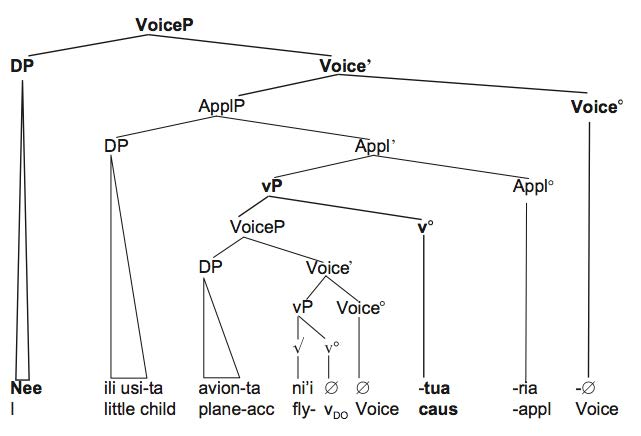
\includegraphics[width=0.7\textwidth]{figs/harley1.jpg}

\ex \begingl
	\gla Nee uka avion-ta ni'i-\textbf{tua}-\underline{tevo}-k//
	\glb I the plane-\gsc{acc} fly-\gsc{caus-caus.indir}-Perf//
	\glft `I had the plane flown (by somebody)'.//
	\endgl
\xe
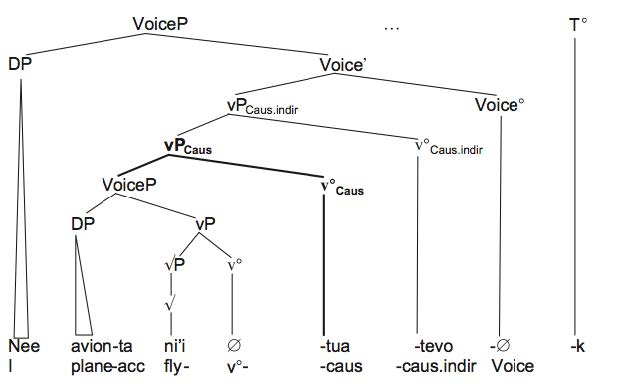
\includegraphics[width=0.7\textwidth]{figs/harley2.jpg}	

	    \subsubsection{Passivized causatives in Hiaki}
When passive is added to \textbf{\emph{–tua}}, the external argument of the caused vP is made the subject of the passive verb, since it is an argument of the causative verb.

\ex \raisebox{-19em}{ 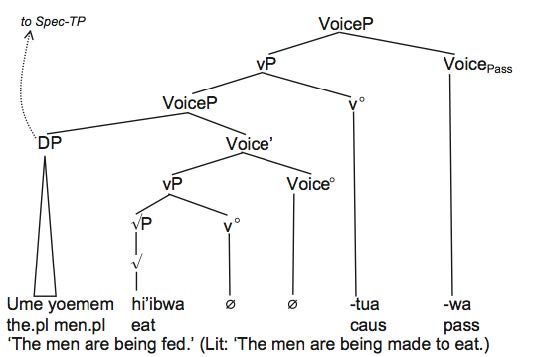
\includegraphics[width=0.7\textwidth]{figs/harley3.jpg} }
\xe

When passive is added to \underline{\emph{-tevo}}, the object of the lower vP is made the subject of the passive, since it is the highest complement of the derived causative verb.
\ex	\raisebox{-14em}{ 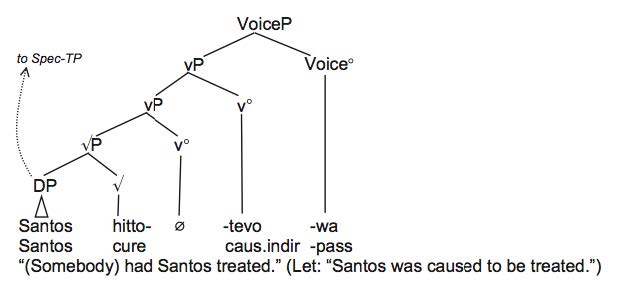
\includegraphics[width=0.8\textwidth]{figs/harley4.jpg} }
\xe




% \begin{mdframed}[hidealllines=true,innerleftmargin=3pt,leftmargin=0pt,innerrightmargin=10pt,rightmargin=-3pt,backgroundcolor=gray!20]
% \textbf{Mystery:} Why does English (and other languages) care about the existence of a complement to the passive verb?
% \pex
% 	\a It was danced all night long.
% 	\a \ljudge{*} There was danced all night long.
% 	\a \ljudge{*} At the party was danced by the children.
% \xe
% \end{mdframed}

    \subsection{Additional phenomena and formal tools}

        \subsubsection{Head movement}
\textbf{Adverbs}
\ex \begingl
		\gla Jean a \fbox{souvent} embrass\'e Pierre//
		\glb Jean has often kissed Pierre//
		\glft `Jean has often kissed Pierre.'//
	\endgl
\xe

\pex
	\a \begingl
		\gla Jean \textbf{embrasse} \fbox{souvent} Pierre//
		\glb Jean kisses often Pierre//
		\glft `Jean often kisses Pierre.'//
	\endgl

	\a \ljudge{*} \begingl
		\gla Jean \fbox{souvent} \textbf{embrasse} Pierre//
		\glb Jean often kisses Pierre//
		\glft (Intended: `Jean often kisses Pierre')//
	\endgl
\xe	
\bigskip

\textbf{Negation}
\ex
	\begingl
		\gla Jean (n')a \fbox{pas} embrass\'e Pierre//
		\glb Jean \phantom{(n')}has not kissed Pierre//
		\glft `Jean has not kissed Pierre.'//
	\endgl
\xe

\pex	
	\a \begingl
		\gla Jean (n')\textbf{embrasse} \fbox{pas} Pierre//
		\glb Jean \phantom{(n')}kisses not Pierre//
		\glft `Jean does not kiss Pierre.'//
	\endgl

	\a \ljudge{*} \begingl
		\gla Jean (ne) \fbox{pas} \textbf{embrasse} Pierre//
		\glb Jean {} not kiss Pierre//
		\glft (Int.~`Jean does not kiss Pierre')//
	\endgl
\xe

Common assumptions:
\begin{itemize} \tightlist
	\item Morphologically complex words are built by head-to-head(-to-head) movement up the tree.
	\item If head-movement adjoins heads to the left of what they're adjoined to, then as you move rightwards, you go higher in scope.
	\item Some prefixes, e.g.~English \emph{re-} and \emph{un-}, would need to head-move from a low position.
\end{itemize}
Not necessarily true! But productive.


    \subsubsection{Cliticization}
In some cases, morphemes seem to be only partially positioned by the syntax.
\begin{itemize} \tightlist
	\item \textbf{Clitics} are positioned with respect to phrases by the syntax.
	\item Their \emph{hosts}---the words with which they are pronounced---appear to be chosen by phonological considerations.
	\item Some clitics seem to lean on neighboring words after positioning via the syntax.
	\item Other clitics infix morphophonologically into constituents they are positioned next to.
\end{itemize}

\textbf{Straightforward clitics}
\ex Queen of England's hat\\
\Tree
[.DP
	\qroof{Queen of England}.DP
	[.D'
		[.D\\\emph{'s} ]
		[.NP\\\emph{hat} ]
	]
]
\xe

\textbf{Phonological attachment}
Where can Bosnian-Croatian-Serbian auxiliares appear?

\pex
	\a \begingl
		\gla koji \textbf{je} \v{c}ovjek koju knjigu kupio?//
		\glb which is man which book bought//
		\glft `Which man bought which book?'//
	\endgl
	
	\a \begingl
		\gla koji \v{c}ovjek \textbf{je} koju knjigu kupio?//
		\glb which man is which book bought//
		\glft `Which man bought which book?'//
	\endgl
\xe

\pex
	\a \begingl
		\gla moja mladja sestra \textbf{\'ce} do\'ci u utorak//
		\glb my younger sister will come on Tuesday//
		\glft `My younger sister will come on Tuesday.'//
	\endgl
	
	\a \begingl
		\gla moja \textbf{\'ce} mladja sestra do\'ci u utorak//
		\glb my will younger sister come on Tuesday//
		\glft `My younger sister will come on Tuesday.'//
	\endgl
\xe
After the first phonological word \textbf{or} first constituent.

\bigskip

Latin:
\pex 
	\a \begingl
		\gla {[} [ bon-i\textipa{:} puer-i\textipa{:} ] [ que [ bon-ae puell-ae ] ] ]//
		\glb good-\gsc{M.PL} boy-\gsc{M.PL} and good\gsc{F.PL} girl-\gsc{F.PL}//
	\endgl
	\a \emph{boni\textipa{:} pueri\textipa{:} bonae-que puellae}
\xe
	

	   \subsubsection{Non-active Voice}
Non-active Voice is often marked by an element external to tense and agreement.
\pex French
	\a \begingl
		\gla Jean a cassé le verre//
		\glb Jean has broken the glass//
		\glft `John has broken the glass.'//
	\endgl
	\a \begingl
		\gla Le verre \textbf{s}'est cass\'e//
		\glb the glass \gsc{SE}=has broken//
		\glft `The glass broke.'//
	\endgl
\xe

\pex Russian
	\a \begingl
		\gla ja zak\'ont\textipa{S}il klas//
		\glb I ended class//
		\glft `I ended the class.'//
	\endgl
	
	\a \begingl
		\gla klas zakont\textipa{S}il\textbf{as\super{j}}//
		\glb class end=\gsc{SJA}//
		\glft `The class was ended', `The class ended.'//
	\endgl
\xe

\ex \begingl
	\gla letom razmer belyx pjaten na Marse umen'\textipa{S}aet\textbf{sja}//
	\glb in-summer size of-white spots on Mars decrease=\gsc{SJA}//
	\glft `In the summer, the size of the white spots on Mars decreases'//
	\endgl
\xe

\pex Icelandic
	\a J\'on se\textbf{st}\\
	`John seats himself' (reflexive)
	\a J\'on gref\textbf{st}\\
	`John gets buried' (passive)
	\a Dyrnar opna\textbf{st}\\
	`The door opens' (unaccusative)
\xe

The external argument is not projected.

Part of the verb and not of the next phonological word.
\pex
	\a \emph{mer-st} [m\textbf{e}r-st] `gets crushed'\\
		\emph{mer storan} [m\underline{e\textipa{:}}r] `crush big'
	\a \emph{gref-st} [kr\textbf{e}f-st] `gets buried'\\
		\emph{gref storan} [gr\underline{e\textipa{:}v}] `bury big'
\xe
\bigskip

Tree: Clitics that originate in the specifier of voice, rather than as the head of voice. They cliticize to the inflected verb.

    \subsection{For reflection}
What does the interaction of argument structure and morphology teach us about the interface between syntax and morphology?


\newpage
\bibliographystyle{linquiry2}
\bibliography{lingxbib}

\end{document}
